%\documentclass[11pt]{article}
%% packages
%\usepackage[french]{babel}
%\usepackage[utf8]{inputenc}
%\usepackage{geometry}
%\usepackage[pdftex]{graphicx}
%\usepackage{graphicx}
%\usepackage{tabularx}
%\usepackage{dsfont}
%\usepackage{multirow}
%\usepackage{amsmath,amsfonts,amssymb}
%\usepackage{subcaption}
%\usepackage{authblk}
%\usepackage{placeins}
%%hyperlinks options
%\usepackage{hyperref}
%\hypersetup{colorlinks=true,linkcolor=blue,filecolor=magenta,urlcolor=cyan,citecolor=cyan}
%%bib options
%\usepackage[backend=biber,style=authoryear,bibstyle=authoryear,natbib=true,
%giveninits=true,uniquename=false,uniquelist=false,% firstinits=false,
%maxcitenames=2,date=year, maxbibnames=99,url=false]{biblatex}
%\geometry{left=20mm, top=20mm, right=20mm}
%%float barrier
%\usepackage{placeins}
% \addbibresource{Thèse.bib}
%\title{Chapitre 4 : Analyse probabiliste des crues du Rhône à Beaucaire du XVI\textsuperscript{ème} siècle à aujourd'hui}
%\author{Mathieu}
%
%
%\begin{document}
%\maketitle
%
%\tableofcontents

\chapter{Analyse probabiliste des crues du Rhône à Beaucaire du XVI\textsuperscript{ème} siècle à aujourd'hui}
\label{chap:ch4}
\newpage

\section{Introduction du chapitre}

	\paragraph{} Un des problèmes majeurs de l'analyse fréquentielle des crues provient de la difficulté à estimer précisément les paramètres de la distribution choisie, notamment à cause de la longueur limitée des chroniques disponibles (\cite{kjeldsen_uncertainty_2011}; \cite{apel_flood_2004}). Cette incertitude d'échantillonnage est d'autant plus grande que la période de retour du quantile estimé est grande devant la longueur de la chronique (i.e. estimer le débit de la crue millénale en se basant sur une chronique de débits maximum annuels de 20 ans). Cette situation est fréquente, notamment en France ou la longueur des chroniques de débit mesurées en continu est en moyenne de l'ordre de 50 ans \citep{le_coz_quantifying_2017}, alors que la plus forte crue connue ou la crue centennale si celle-ci est supérieure est la référence en terme de niveau de protection dans les communes. En Angleterre, il est déconseillé d'estimer des quantiles de période de retour supérieure à la moitié de la longueur de la chronique continue utilisée \citep{whs_flood_2008}. Cependant, est possible de réduire l'incertitude d'échantillonnage en élargissant le jeu de données de diverses manières.
	 
	\paragraph{}Tout d'abord, il existe des méthodes permettant d'élargir spatialement le jeu de données sous certaines conditions, en faisant par exemple l'hypothèse que la distribution des crues est homogène au sein d'une région définie à un facteur d'échelle près (\cite{hosking_regional_1997}; \cite{gaume_bayesian_2010}; \cite{viglione_flood_2013}; \cite{nguyen_regional_2014}) ou bien en utilisant un modèle qui prend en compte les dépendances spatiales entre stations (\cite{kjeldsen_exploratory_2009}; \cite{renard_bayesian_2011}; \cite{sun_general_2014}). Néanmoins, il semble inapproprié d'appliquer une analyse régionale à la station du Rhône à Beaucaire, la notion de région homogène ayant peu de sens ici étant donné la taille du bassin versant et les nombreuses influences hydro-climatiques qui impactent la distribution des crues.
	
	\paragraph{} Une autre méthode populaire consiste à élargir temporellement le jeu de données disponible en utilisant des données anciennes, pouvant être d'origine et de nature variées. Le cas idéal, décrit dans le chapitre \ref{chap:ch3}, illustre la possibilité d'exhumer des enregistrements continus, antérieurs aux données disponibles dans les bases de données. Dans cette situation, l'exhaustivité des débits maximum annuels est garantie et le principal défi méthodologique est de considérer les diverses sources d'incertitudes. Plus généralement, les données historiques disponibles ne sont pas continues et peuvent prendre des formes variées et donc nécessiter des traitements statistiques différents. Il peut s'agir de témoignages (\cite{pichard_les_1995}; \cite{kjeldsen_documentary_2014}), de repères de crues (\cite{parkes_defining_2016}; \cite{piotte_collection_2016}; \cite{engeland_new_2020}; \cite{medd_reperes_2023}), de reconstructions de crues pré-historiques (ou paléocrues) issues de divers proxys tels que les dépôts sédimentaires ou les cernes des espèces végétales ripariennes (\cite{stedinger_flood_1986}; \cite{benito_use_2004}; \cite{dezileau_multidating_2014}; \cite{st_george_paleofloods_2020}; \cite{engeland_new_2020}). L'utilisation des données historiques pour l'analyse fréquentielle n'est pas récente, en témoignent par exemple les travaux de \citet{benson_use_1950} ou de \citet{hirsch_plotting_1987} qui se consacraient principalement au placement des crues sur les courbes de fréquence. Les travaux de \citet{stedinger_flood_1986} ont ensuite ouvert la voie à l'inclusion de ces données dans l'estimation de la distribution des crues via l'utilisation de l'estimateur du maximum de vraisemblance et les méthodes Monte-Carlo. De nombreuses méthodes existent à ce jour pour inclure les données historiques à l'analyse fréquentielle des crues. Parmi elles, les méthodes d'inférence bayésienne permettent d'inclure des données de nature diverse via l'utilisation de la fonction de vraisemblance (\cite{stedinger_flood_1986}; \cite{kuczera_comprehensive_1999}) et l'utilisation d'algorithmes MCMC (\cite{reis_bayesian_2005}; \cite{renard_application_2006}). La plupart des études récentes qui valorisent les données historiques soulignent qu'une prise en compte complète des incertitudes est nécessaire (\cite{neppel_flood_2010}; \cite{parkes_defining_2016}).
	
	\paragraph{} Les données de crues historiques ne sont généralement pas continues et concernent des crues d'une magnitude suffisante pour avoir par exemple laissé une trace dans les écrits ou pour avoir mérité l'installation d'un repère de crue. Le dénominateur commun du traitement statistique de ces données de forme variée est le seuil de perception (\cite{gerard_probability_1979}; \cite{stedinger_flood_1986}). Il s'agit ici de faire l'hypothèse que toutes les crues ayant dépassé ce seuil de perception ont laissé une trace, ce qui garantit l'exhaustivité du recensement des crues historiques. Le corolaire à cette idée est que, pour toutes les années de la période historique sans mention de crue, on fait l'hypothèse que le débit maximum annuel a été inférieur au seuil de perception. Il est parfois possible de reconstituer le débit des crues historiques supérieures au seuil de perception, notamment via l'utilisation de modèles hydrauliques (\cite{neppel_flood_2010}, \cite{machado_flood_2015}). Il n'est cependant pas obligatoire de connaitre le débit des crues historiques. La seule connaissance du nombre de crues ayant dépassé le seuil de perception est suffisante pour exploiter les données via l'utilisation de la loi binomiale, tel que décrit par \citet{stedinger_flood_1986} ou \citet{payrastre_usefulness_2011}. Le seuil de perception est un concept empirique qui ne prend une signification physique que dans certaines situations. Par exemple, imaginons une station hydrométrique dont la section n'a pas évolué au cours du temps et pour laquelle les débordements surviennent toujours au delà d'un même débit. Ces débordements (par exemple au-dessus d'une digue qui n'a subi aucune modification au cours du temps) laissent systématiquement une trace dans les écrits ou sur des infrastructures (marques de crue) suite aux dommages occasionnés. Cette situation parfaite existe rarement et le concept de seuil de perception peut être mis à mal par une variabilité temporelle de la perception des crues par les populations ripariennes. Néanmoins, le seuil de perception est dans la grande majorité des cas supposé parfaitement connu, bien que la sensibilité des résultats au choix du seuil de perception soit parfois explorée (\cite{stedinger_flood_1986}, \cite{viglione_flood_2013}; \cite{macdonald_reassessing_2014}; \cite{payrastre_usefulness_2011}). Seuls les travaux de \citet{parkes_defining_2016} semblent avoir considéré une incertitude du seuil de perception, et ce uniquement dans des cas où le débit des crues historiques est connu. Néanmoins, le seuil de perception n'apparait pas dans la formulation de la vraisemblance, et les distributions a priori utilisées ne sont pas explicitées. Il est pourtant possible d'intégrer directement l'incertitude du seuil de perception, l'incertitude des quantiles estimés étant ainsi impactée en fonction de la méconnaissance du seuil de perception. 

	\paragraph{} Le concept de seuil de perception est accompagné de la définition de la durée de la période historique. La date qui marque le début de cette période historique (date à partir de laquelle le seuil de perception est actif) est complexe et même parfois impossible à déterminer. Pourtant, à l'instar du seuil de perception, cette durée est généralement considérée comme étant parfaitement connue dans la littérature. Définir le début de la période historique à la date de première crue connue est dangereux, cela peut mener à une sous-estimation de la durée de la période historique et donc à une sur-estimation des quantiles de crue. Pour pallier à ce problème, \citet{prosdocimi_german_2018} propose une comparaison de méthodes pour estimer la durée de période historique lorsque celle ci n'est pas connue. La prise en compte de ce problème au sein même du modèle probabiliste semble possible mais n'a pas été étudié dans la littérature. Cependant, il semble légitime que l'incertitude des quantiles estimés soit impactée par la méconnaissance autour de cette durée. 
	
	\paragraph{} Même si les débits de la période continue sont généralement bien mieux connus que ceux de la période historique, il existe une incertitude autour de ces données. Cette incertitude est pourtant souvent négligée dans le cas de l'utilisation de données historiques. Seuls quelques travaux proposent de la prendre en compte : \citet{parkes_defining_2016} considèrent l'incertitude autour de la période continue via l'utilisation d'un pourcentage d'erreur fixe, et \citet{neppel_flood_2010} via l'utilisation de modèles d'erreur plus élaborés. Dans le cas de la station du Rhône à Beaucaire, l'incertitude des débits de la période continue a été minutieusement déterminée pour chacune des sources existantes et propagée aux débits maximum annuels (chapitre \ref{chap:ch3}). Cette prise en compte des incertitudes hydrométriques semblait ici indispensable compte tenu de la longueur exceptionnelle de la chronique et de l'utilisation de données continues particulièrement anciennes. Cette incertitude pourra être propagée aux quantiles estimés dans ce chapitre via l'utilisation de procédures Monte-Carlo, de manière similaire à la propagation réalisée au chapitre \ref{chap:ch3}.
	
	\paragraph{} Ce chapitre présente un modèle probabiliste qui utilise le nombre de dépassements d'un seuil de perception pour l'analyse fréquentielle et qui prend en compte l'incertitude des débits de la période continue. Un des objectifs majeurs de ce chapitre est de reconnaitre la nature imparfaitement connue du seuil de perception et de la durée de la période historique en en faisant des paramètres a part entière 	du modèle probabiliste. Cet objectif est exploré grâce à l'utilisation d'un jeu de données continues de 205 ans à Beaucaire. Ce jeu de données est artificiellement dégradé afin de se replacer dans le contexte d'un échantillon mixte, tout en connaissant parfaitement les caractéristiques de l'échantillon historique afin de pouvoir évaluer les résultats des modèles. L'apport de la connaissance du débit des crues historiques est également exploré et comparé à la seule connaissance du nombre de dépassement du seuil de perception. Ces mêmes modèles sont ensuite appliqués à un échantillon mixte de 1500 à 2020 à Beaucaire pour lequel l'impact des différentes incertitudes sur les quantiles est discuté. 
	
	\paragraph{} Les méthodes d'analyse fréquentielle des crues historiques sont présentées dans une première partie (section \ref{sec:MethodoCh3}). Les données disponibles à Beaucaire sont présentées et l'homogénéité de ces échantillons est vérifiée (section \ref{sec:dataBcr}). Les modèles sont ensuite appliqués à un échantillon dégradé, puis à l'intégralité de l'échantillon de crues du Rhône à Beaucaire (section \ref{sec:applicationBcr}). Les résultats sont ensuite discutés en section \ref{sec:Discussion}.	
		
		
\section{Méthodes d'analyse probabiliste d'un échantillon mixte de crues}
\label{sec:MethodoCh3}
	
	\subsection{Concepts de base et hypothèses}
	\label{subsec:conceptsdebase}
	
	\textcolor{red}{premier paragraphe doublon avec l'intro, a effacer ou rephraser?}
	\paragraph{} L'utilisation d'occurrences de crues historiques pour l'analyse fréquentielle nécessite a minima l'hypothèse suivante : toutes les crues ayant dépassé une certaine magnitude ont laissé une trace dans les archives ou les mémoires. On nommera cette magnitude : "seuil de perception". Cela implique que pour toutes les années de la période historique sans mention de crue, on fait l'hypothèse que le débit inconnu a été inférieur au seuil de perception. Aussi, l'échantillon des crues supérieures au seuil de perception est supposé exhaustif. Il existe des méthodes d'analyse pour lesquelles il n'est pas nécessaire de connaitre précisément le débit des événements supérieurs au seuil de perception (voir notamment \citet{stedinger_flood_1986}). Le nombre de dépassements d'un seuil de perception pour une durée donnée est une information qui peut être exploitée en l'état. Ainsi, il faut considérer un échantillon mixte, composé d'une part de débits enregistrés en continu et d'autre part d'un nombre d'occurrences de crues supérieures à un seuil de perception. 
			
		\paragraph{} De manière similaire au chapitre \ref{chap:ch3}, on suppose que le débit maximum annuel des périodes continues et historiques $Q$ est une variable aléatoire $iid$ qui suit une distribution GEV, de paramètres $\boldsymbol{\theta} = (\mu,\sigma,\xi)$ (respectivement : position, échelle, forme). Pour simplifier, on suppose ici que le paramètre de forme $\xi$ est différent de zéro (loi de Gumbel). Ainsi, on a la fonction de répartition de la GEV : $F(x;\boldsymbol{\theta}) = e^{-(1-\xi(\frac{x - \mu}{\sigma}))^{1/\xi}}$. Lorsque le paramètre de forme est strictement positif ($\xi > 0$), on se trouve dans le cas "loi de Weibull" avec une borne supérieure et des quantiles inférieurs à ceux d'une loi de Gumbel. Dans le cas contraire ($\xi < 0$), il s'agit du cas "loi de Fréchet" de la distribution GEV. Les débits de l'échantillon de maximum annuels enregistrés en continu pendant $j$ années $\boldsymbol{q}= (q_t)_{t=1,...,j}$ sont ici supposés parfaitement connus et dans un premier temps non affectés d'une quelconque incertitude. L'échantillon historique est composé de $k$ événements ayant dépassé le seuil de perception $S$ sur une période de $n$ années. Le seuil de perception n'a donc pas été dépassé pour les $n-k$ années restantes. La probabilité de dépassement du seuil peut s'écrire :
		
		\begin{equation}
			\pi = \biggl( 1 - F(S;\boldsymbol{\theta})\biggl) = 1 - e^{-\biggl(1-\xi\bigl(\frac{S-\mu}{\sigma}\bigl)\biggl)^{1/\xi} }		
		\end{equation}
			 
	On suppose que $k$, le nombre de dépassements du seuil de perception, peut être estimé par une loi binomiale de paramètres $n$ et $\pi$, soit $\mathcal{B}(n,\pi)$. On peut alors écrire la fonction de vraisemblance (équation \ref{eq:Gev_Binom}) qui est fonction d'un échantillon mixte de données composé des débits maximum annuels de la période continue $(q_t)_{t=1,...,j}$ et du nombre de dépassements du seuil de perception $k$ durant la période historique $n$ :
		
			\begin{equation}
			L(\boldsymbol{\theta} ; \boldsymbol{q}, k) = \underbrace{\prod_{t=1}^j f\left(q_t;\boldsymbol{\theta}\right)}_{\mathrm{a}} \underbrace{\left\{\left(\begin{array}{l}
			n \\
			k
			\end{array}\right) F\left(S;\boldsymbol{\theta}\right)^{n-k}\left[1-F\left(S;\boldsymbol{\theta}\right)\right]^k\right\}}_{\mathrm{b}} \\
			\label{eq:Gev_Binom}
			\end{equation}
			
			Ici, le terme \textit{$\mathrm{(a)}$} représente la vraisemblance pour les données continues et le terme \textit{$\mathrm{(b)}$} la vraisemblance pour les données historiques. L'application de la formule de Bayes permet de calculer la distribution a posteriori des paramètres $\boldsymbol{\theta}$ sachant les données :
			
			\begin{equation}
				p(\boldsymbol{\theta} \mid \boldsymbol{q},k) \propto L(\boldsymbol{\theta};\,\boldsymbol{q},k) p(\boldsymbol{\theta})
				\label{eq:BayesBinom}
			\end{equation}
	
		Le terme $p(\boldsymbol{\theta})$ représente ici la distribution a priori des paramètres qu'il faudra éliciter. La distribution a posteriori est explorée via une méthode bayésienne MCMC \citep{renard_application_2006}. Cette distribution a posteriori représente l'incertitude d'échantillonnage du modèle par $r$ jeux de paramètres : $\boldsymbol{\Theta} = (\boldsymbol{\theta_1},...,\boldsymbol{\theta_r})$. Le jeu de paramètres qui maximise la distribution a posteriori est appelé maxpost et s'écrit $\boldsymbol{ \hat{\theta} }$. Pour l'ensemble des simulations du présent chapitre, les a priori des paramètres de la distribution GEV seront les suivants : distribution plate (uniforme et très peu informative) pour $\mu$ et $\sigma$, et distribution gaussienne de moyenne zéro et d'écart type 0.2 pour $\xi$. Cet a priori du paramètre de forme est notamment cohérent avec les suggestions de \citet{martins_generalized_2000}.
	
	
%	\paragraph{Description difficultés de détermination du seuil et durée historique}
%	Complexité de déterminer le seuil\\
%	Complexité de déterminer la durée de la période historique \citep{prosdocimi_german_2018}). 			Attention aux confusions entre date de début de la période et durée de la période. \\

	
	\subsection{Propagation de l'incertitude hydrométrique des mesures systématiques (modèle A)}
	\label{subsec:modA}
	
	\paragraph{} Dans la section précédente, l'incertitude des débits maximum annuels de la période continue est supposée négligeable. Cette incertitude pouvant atteindre 30 \% à Beaucaire (chapitre \ref{chap:ch3}), il semble pragmatique de la considérer. Comme décrit dans le chapitre \ref{chap:ch3}, cette incertitude hydrométrique est représentée par $s = 500$ réalisations : $(q_t^{(i)})_{t=1,...,j;\,i=1,...,s}$. Elle peut être propagée aux estimations des paramètres de l'équation \ref{eq:Gev_Binom} en estimant un jeu de paramètres pour chacune des $s$ réalisations, soit $(\boldsymbol{\theta}
	^{(i)})_{i=1,...,s}$. Au total, $r \times s$ jeux de paramètres sont estimés et représentent l'effet combiné de l'incertitude d'échantillonnage et de l'incertitude hydrométrique des données continues, on a donc $(\boldsymbol{\theta}^{(i)}_p)_{p=1,...,r;\, i=1,...,s}$. Le jeu de paramètres le plus probable est calculé en utilisant l'échantillon maxpost de débits maximum annuels (issu du \ref{chap:ch3} sur lequel on estime le jeu de paramètres maxpost de l'équation \ref{eq:Gev_Binom}. Le modèle décrit ci-dessus sera appelé "modèle A". La propagation des incertitudes hydrométriques de la période continue telle que décrite ici sera effectuée similairement pour les trois modèles définis dans les sections suivantes.
	
	\subsection{Seuil de perception incertain (modèle B)}
	\label{subsec:modB}
	
		\paragraph{}
		Afin de considérer dans le modèle probabiliste une prise en compte pragmatique de la méconnaissance du seuil de perception, il est possible de considérer ce seuil comme étant un paramètre à part entière du modèle. Un seul seuil de perception est ici considéré pour l'ensemble de l'échantillon et sa valeur est incertaine et est déterminée par le modèle. L'impact de la méconnaissance du seuil est ainsi répercuté sur l'incertitude des résultats. Dans la section précédente, le seuil de perception faisait déjà partie du modèle (équation \ref{eq:Gev_Binom}), mais sa valeur était supposée connue, ce qui n'est ici plus le cas. La vraisemblance s'écrit alors : 
		
				\begin{equation}
				L(\boldsymbol{\theta}, S ; \boldsymbol{q}, k) =\prod_{t=1}^j f\left(q_t;\boldsymbol{\theta}\right) \left\{\left(\begin{array}{l}
				n \\
				k
				\end{array}\right) F\left(S;\boldsymbol{\theta}\right)^{n-k}\left[1-F\left(S;\boldsymbol{\theta}\right)\right]^k\right\} \\
				\label{eq:Gev_Binom_uS}
				\end{equation}
				
		On peut alors écrire une nouvelle distribution a posteriori : 			
				
				\begin{equation}
					p(\boldsymbol{\theta}, S \mid \boldsymbol{q},k) \propto L(\boldsymbol{\theta},S;\,\boldsymbol{q},k) p(\boldsymbol{\theta},S)
					\label{eq:Bayes_uS}
				\end{equation}
			
		La distribution des paramètres a posteriori de ce modèle reflètent l'incertitude hydrométrique de la période continue, l'incertitude d'échantillonnage, ainsi que l'incertitude du seuil de perception. Ce modèle sera nommé "modèle B" dans les sections suivantes. Il est ici nécessaire de spécifier une distribution a priori du seuil de perception qui reflète la connaissance, qu'elle soit très partielle ou relativement précise, de ce paramètre. 

	\subsection{Durée de la période historique incertaine (modèle C)}
	\label{subsec:modC}
	
		\paragraph{}
		L'équation \ref{eq:Gev_Binom} repose à la fois sur le fait que le seuil de perception $S$ et la durée de la période historique $n$ sont connus. De la même manière que décrit à la section précédente pour le seuil, la durée (et donc l'année qui marque le début) de la période historique peut être complexe à déterminer. Généralement, la date qui marque la fin de la période historique est parfaitement connue, car elle correspond également au début des enregistrements continus. En revanche, la date du début de l'échantillon historique (que l'on appellera $t^{*}$), à partir de laquelle toutes les crues supérieures au seuil de perception seront connues, correspond à une période lointaine et relativement mal connue de l'échantillon historique. Ainsi, nous proposons ici de considérer la durée de la période historique $n$ comme étant un paramètre à part entière du modèle probabiliste. Le seuil de perception est en revanche supposé parfaitement connu dans ce cas de figure. La vraisemblance s'écrit alors : 
		 
				\begin{equation}
				L(\boldsymbol{\theta}, n ; \boldsymbol{q}, k) = \prod_{t=1}^j f\left(q_t;\boldsymbol{\theta}\right) \left\{\left(\begin{array}{l}
				n \\
				k
				\end{array}\right) F\left(S;\boldsymbol{\theta}\right)^{n-k}\left[1-F\left(S;\boldsymbol{\theta}\right)\right]^k\right\} \\
				\label{eq:Gev_Binom_uN}
				\end{equation}
				
		On peut alors exprimer une nouvelle distribution a posteriori :
		
				\begin{equation}
					p(\boldsymbol{\theta}, n \mid \boldsymbol{q},k) \propto L(\boldsymbol{\theta},n;\,\boldsymbol{q},k) p(\boldsymbol{\theta},n)
					\label{eq:Bayes_uN}
				\end{equation}
			
		La méconnaissance de la durée de la période historique $n$ est donc prise en compte dans le modèle et a un impact sur l'incertitude des résultats. Ce modèle sera nommé "modèle C" dans les sections suivantes. Une distribution a priori reflétant la connaissance partielle autour de la durée de la période historique devra être élicitée. 
	
	\subsection{Seuil de perception et durée de la période historique incertains (modèle D)}
	\label{subsec:modD}	
	
	\paragraph{}
	Le seuil de perception $S$ et la durée de la période historique $n$ étant par définition reliés (un seuil de perception étant valide sur une durée donnée) on peut construire un modèle qui représente en même temps la méconnaissance autour de ces deux paramètres. La vraisemblance de ce modèle s'écrit :  
	
					\begin{equation}
			L(\boldsymbol{\theta}, S, n ; \boldsymbol{q}, k) = \prod_{t=1}^j f\left(q_t;\boldsymbol{\theta}\right) \left\{\left(\begin{array}{l}
			n \\
			k
			\end{array}\right) F\left(S;\boldsymbol{\theta}\right)^{n-k}\left[1-F\left(S;\boldsymbol{\theta}\right)\right]^k\right\} \\
			\label{eq:Gev_Binom_SN}
			\end{equation}
		
		On peut exprimer la vraisemblance du modèle telle que :
					
			\begin{equation}
				p(\boldsymbol{\theta}, S, n \mid \boldsymbol{q},k) \propto L(\boldsymbol{\theta},S, n;\,\boldsymbol{q},k) p(\boldsymbol{\theta},S, n)
				\label{eq:Bayes_uSN}
			\end{equation}

	Ce modèle pour lequel $S$ et $n$ sont incertains sera nommé "modèle D" dans les sections suivantes. 
	
	\subsection{Débit des crues historiques compris dans un intervalle (modèle E)}
	\label{subsec:modE}	
		
	\paragraph{} Dans certains cas, le débit des crues historiques supérieures au seuil de perception est connu. De façon similaire au modèle binomial décrit précédemment, on peut faire l'hypothèse que le débit maximum annuel de toutes les années de la période historique sans mention de crues est inférieur au seuil de perception. Le débit des crues historiques peut ensuite être pris en compte dans le modèle probabiliste décrit par \citet{stedinger_flood_1986}. Il est également possible de considérer que le débit des crues historiques n'est pas parfaitement connu, mais qu'il est compris dans un intervalle de confiance. Plusieurs exemples d'un tel modèle existent dans la littérature (par exemple : \citet{payrastre_usefulness_2011} ou \citet{parkes_defining_2016}). La vraisemblance d'un tel modèle peut s'écrire : 

		\begin{equation}
					L(\boldsymbol{\theta} ; \boldsymbol{q}, \boldsymbol{y}) =\prod_{t=1}^j f\left(q_t;\boldsymbol{\theta}\right) \prod_{i=1}^k \left[F(y_{i}^{sup},\boldsymbol{\theta} ) - F(y_i^{inf},\boldsymbol{\theta})\right]  F\left(S;\boldsymbol{\theta}\right)^{n-k}
		\label{eq:Censure}
		\end{equation}
					
		\paragraph{}où $q_t$ correspond aux $j$ crues de la période continue et $y_i$ aux $k$ crues de la période historique dont le débit est compris dans l'intervalle d'incertitude à 95\% $\left[y_i^{inf} ; y_i^{sup}\right]$. La distribution a posteriori du modèle s'écrit alors : 
				
		\begin{equation}
			p(\boldsymbol{\theta} \mid \boldsymbol{q},\boldsymbol{y}) \propto L(\boldsymbol{\theta};\,\boldsymbol{q},\boldsymbol{y})p(\boldsymbol{\theta})
		\label{eq:Bayes_Censure}
		\end{equation}

	\paragraph{} Ici, seuil de perception et durée de la période historique sont supposés parfaitement connus. Ce modèle sera nommé "modèle E" dans les sections suivantes. Ici aussi, l'incertitude des débits de la période continue est propagée tel que décrit dans la section \ref{sec:MethodoCh3}. On pourra comparer les quantiles obtenus avec le modèle E pour lequel le débit des crues historiques est connu (dans un intervalle), avec les résultats des modèles binomiaux pour lesquels seul le nombre de dépassements $k$ du seuil de perception est connu.
	

	\subsection{Distribution empirique d'un échantillon mixte}
	\label{subsec:DistEmpirique}
	
		\paragraph{} Le classement en fréquence des crues dans le cas d'un échantillon mixte peut poser problème, notamment quand le débit des crues historiques n'est pas connu, n'ayant d'autre information que le dépassement d'un seuil de perception. \citet{hirsch_probability_1987} propose une méthode pour le classement en fréquence d'un échantillon mixte quand le débit des crues est connu. Pour un échantillon continu de crues classé par valeurs décroissantes : $q(1) \geq ... \geq q(j)$, la fréquence empirique au dépassement s'écrit : $f_i = \frac{i-\alpha}{j+1-2\alpha}$. Nous prenons ici $\alpha = 0.5$ \citep{hazen_storage_1914}. Pour un échantillon mixte composé d'un échantillon continu de $j$ débits maximum annuels et de $k$ crues historiques supérieures à un seuil $S$ couvrant $n$ années, il faut raisonner sous la forme de deux sous-échantillons. Le nombre de crues supérieures au seuil $S$ sur la période complète est ici noté $N_S$, et la durée de la période complète correspond à $j + n$ années. On a d'après \citet{hirsch_probability_1987} :
		
		\begin{equation}	
		f_i = \begin{cases}\dfrac{i-\alpha}{N_S+1-2 \alpha} \dfrac{N_S}{j+n}, & i=1, \ldots, N_S \\ \dfrac{N_S}{j+n}+\dfrac{j+n-N_S}{j+n} \dfrac{(i-N_S-\alpha)}{(j-N_S+1-2\alpha)}, & i=N_S+1, \ldots, j+k\end{cases}
		\label{eq:FreqHisto}	
		\end{equation}
%	
%		\begin{equation}	
%		P(\boldsymbol{Q} > q(i)) = \begin{cases}\frac{i-\alpha}{NS+1-2 \alpha} \frac{NS}{j+n}, & i=1, \ldots, NS \\ \frac{NS}{j+n}+\frac{j+n-NS}{j+n} \frac{(i-NS-\alpha)}{(j-NS+1-2\alpha)}, & i=NS+1, \ldots, j+k\end{cases}
%		\label{eq:FreqHisto}	
%		\end{equation}
%		
	
	\paragraph{} Lorsque le débit des crues historiques est connu, on peut classer l'ensemble des crues supérieures au seuil (de la période continue et historique) par ordre décroissant en leur attribuant le rang $i$. Lorsque le débit des crues historiques n'est pas connu, il n'est pas possible de classer cet échantillon. Une manière de contourner ce problème est de tirer aléatoirement le rang $i$ de l'ensemble des crues supérieures au seuil dans l'intervalle entier $\left[1;N_S\right]$. Ce classement est aléatoire, mais il permet d'affecter une fréquence empirique aux crues. Ainsi, on peut comparer la fréquence empirique des observations de crues aux ajustements statistiques décrits dans les sections précédentes afin de vérifier leur cohérence. 
		
		
\section{Données disponibles}
\label{sec:dataBcr}

	\subsection{Échantillon mixte de crues du Rhône à Beaucaire}
	\paragraph{} L'échantillon de crues du Rhône à Beaucaire est constitué de deux types de données : premièrement, un échantillon continu de débits maximum annuels mesurés de 1816 à 2020. Ces débits ont été estimés au chapitre \ref{chap:ch3} et leur incertitude hydrométrique est représentée par 500 réalisations de l'échantillon. Deuxièmement, une collection de témoignages de crues historiques de 1500 à 1816, tirés de la base HISTRHÔNE et classées en deux catégories tel que décrit au chapitre \ref{chap:ch2}. Les seuils de perception correspondant aux deux échantillons ne sont pas précisément connus, mais on suppose que le seuil $S3$ qui correspond aux crues des catégories C3 et C4 se situe aux alentours de 7000 $m^3/s$, et le seuil $S4$ qui correspond aux crues de la catégorie C4 uniquement se situe aux alentours de 9000 $m^3/s$ (valeur définies au chapitre \ref{chap:ch2}). La figure \ref{fig:EchMixte} présente l'ensemble des données disponibles. 
	
	\begin{figure}[h]
		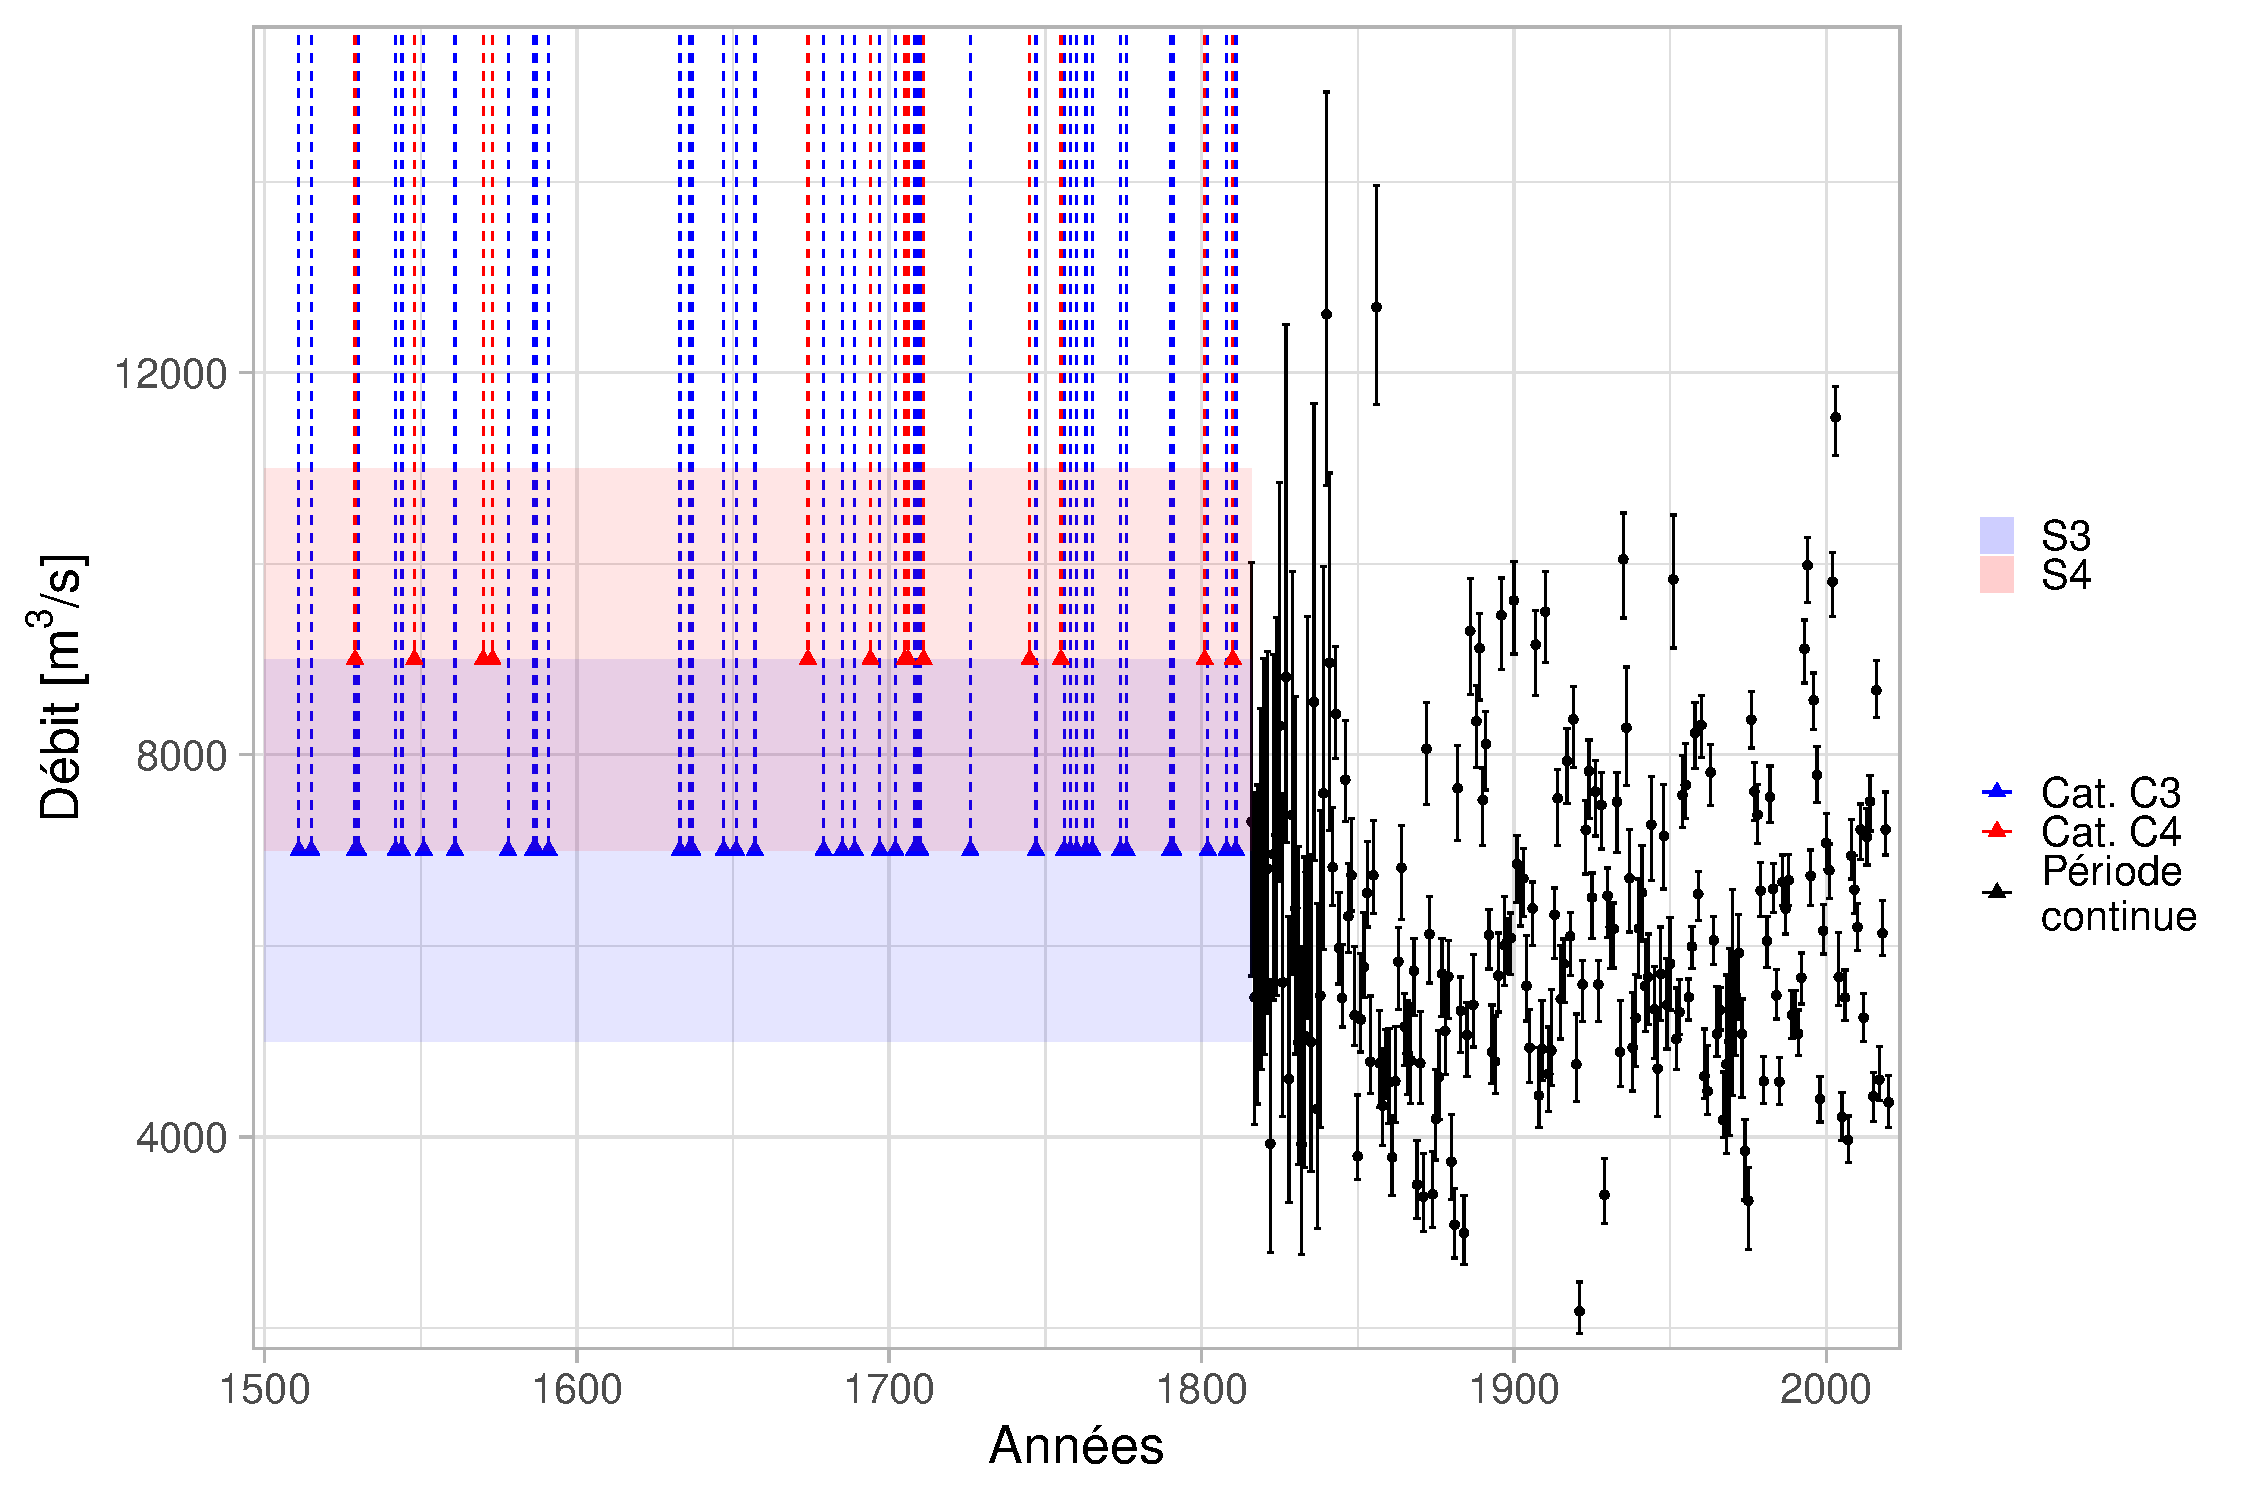
\includegraphics[width=.9\linewidth]{Chapitre4/Figures/EchMixteBcr.pdf}	
		\caption{Échantillon de crues du Rhône à Beaucaire. L'incertitude à 95\% autour des seuils de perception est représentée par les bandeaux bleu et rouge ("S3" et "S4)}
		\label{fig:EchMixte}
	\end{figure}
	

	\subsection{Homogénéité des données}
	\label{subsec:homog}
	\paragraph{} L'homogénéité des données est un pré-requis essentiel à l'analyse fréquentielle des crues en contexte stationnaire, car cette dernière repose sur l'hypothèse que les variables étudiées sont $iid$ (indépendantes et identiquement distribuées). C'est-à-dire que la distribution des crues ne change pas dans le temps et qu'une même distribution peut être utilisée pour modéliser les crues du XVI\textsuperscript{ème} et du XXI\textsuperscript{ème} siècle. Étant donné que deux types d'échantillons sont ici utilisés, deux types de tests statistiques sont appliqués dans les sections suivantes pour étudier l'homogénéité de ces données. 

	\subsubsection{Données continues}
	
	\paragraph{} Trois tests seront utilisés pour qualifier l'homogénéité de l'échantillon de données continues : le test de \citet{pettitt_non-parametric_1979} et la procédure de segmentation développée par \citet{darienzo_detection_2021-1} qui permettent de détecter des ruptures dans les séries temporelles, ainsi que le test de Mann-Kendall (\cite{mann_nonparametric_1945}; \cite{kendall_rank_1948}) qui permet de détecter l'existence de tendances. Les ruptures sont des changements soudains (i.e. les données ont une distribution différente avant et après un instant $t$, par exemple suite à un changement d'instrumentation), tandis que les tendances représentent des changements progressifs dans la distribution des données au cours du temps (par exemple : un changement progressif des conditions d'écoulement du bassin versant). Parmi ces trois tests, seule la procédure de segmentation de \citet{darienzo_detection_2021-1} permet de considérer l'incertitude des données d'entrée (déterminée au chapitre \ref{chap:ch3}).
	
	\paragraph{} La p-value des tests de Pettitt et Mann-Kendall appliqués à la série maxpost des débits maximum annuels à Beaucaire est respectivement de 0.15 et 0.41. Au risque d'erreur 5\%, on peut conclure qu'il n'existe pas de tendance ou de rupture dans la série. Il faut cependant s'assurer que ce résultat est toujours vrai lorsque l'on considère les incertitudes de la série.
			
	\paragraph{} L'application de la procédure de segmentation de \citet{darienzo_detection_2021-1} à la série de débits maximum annuels avec incertitude a conclu que le nombre optimal de segments pour la chronique de Beaucaire était de 1, et ce quel que soit le critère de segmentation considéré (AIC, BIC, HQC ou DIC). On peut ainsi conclure qu'aucune rupture n'existe dans les données. L'échantillon de données continues peut être considéré homogène suite aux tests statistiques réalisés. 
	
%	\paragraph{} Afin de d'étudier l'existence de tendances dans la série en considérant les incertitudes, le test de Mann-Kendall a été appliqué aux 500 réalisations possibles. Seulement 20\% des 500 p-values calculées sont inférieures à 0.05. Au risque d'erreur 5\%, on peut alors conclure que seulement 20\% des 500 réalisations de la série comportent une tendance. On peut calculer une valeur théorique ... A quelle valeur faudrait-il s'attendre pour considérer que c'est homogène (Benjamin ?) 

		
	\subsubsection{Données historiques}
	
	\paragraph{} Les données pré-enregistrements continus (ou historiques) utilisées ici prennent la forme d'occurrences de crues supposées supérieures à un seuil de perception. Comme décrit par \citet{lang_towards_1999}, la fréquence des occurrences de crues supérieures à un seuil est supposée suivre un processus de Poisson. Afin de vérifier l'homogénéité des occurrences de crues, il est possible de calculer un intervalle de confiance autour du nombre cumulé de crues découlant du processus de Poisson. Si les occurrences de crues cumulées "sortent" de cet intervalle de confiance, alors leur fréquence d'occurrence est supposée non-stationnaire. 
	
	\paragraph{} Ces intervalles de confiance ont été calculés pour l'échantillon de crues pré-enregistrements continus du Rhône à Beaucaire. La période historique est supposée débuter en 1500 et se termine à l'année des premiers enregistrements continus de hauteur d'eau, en 1816. Les deux échantillons testés ici reflètent deux seuils de perception, $S3$ et $S4$, et on a $S3 < S4$. 

	\begin{figure}[h]
		\centering
		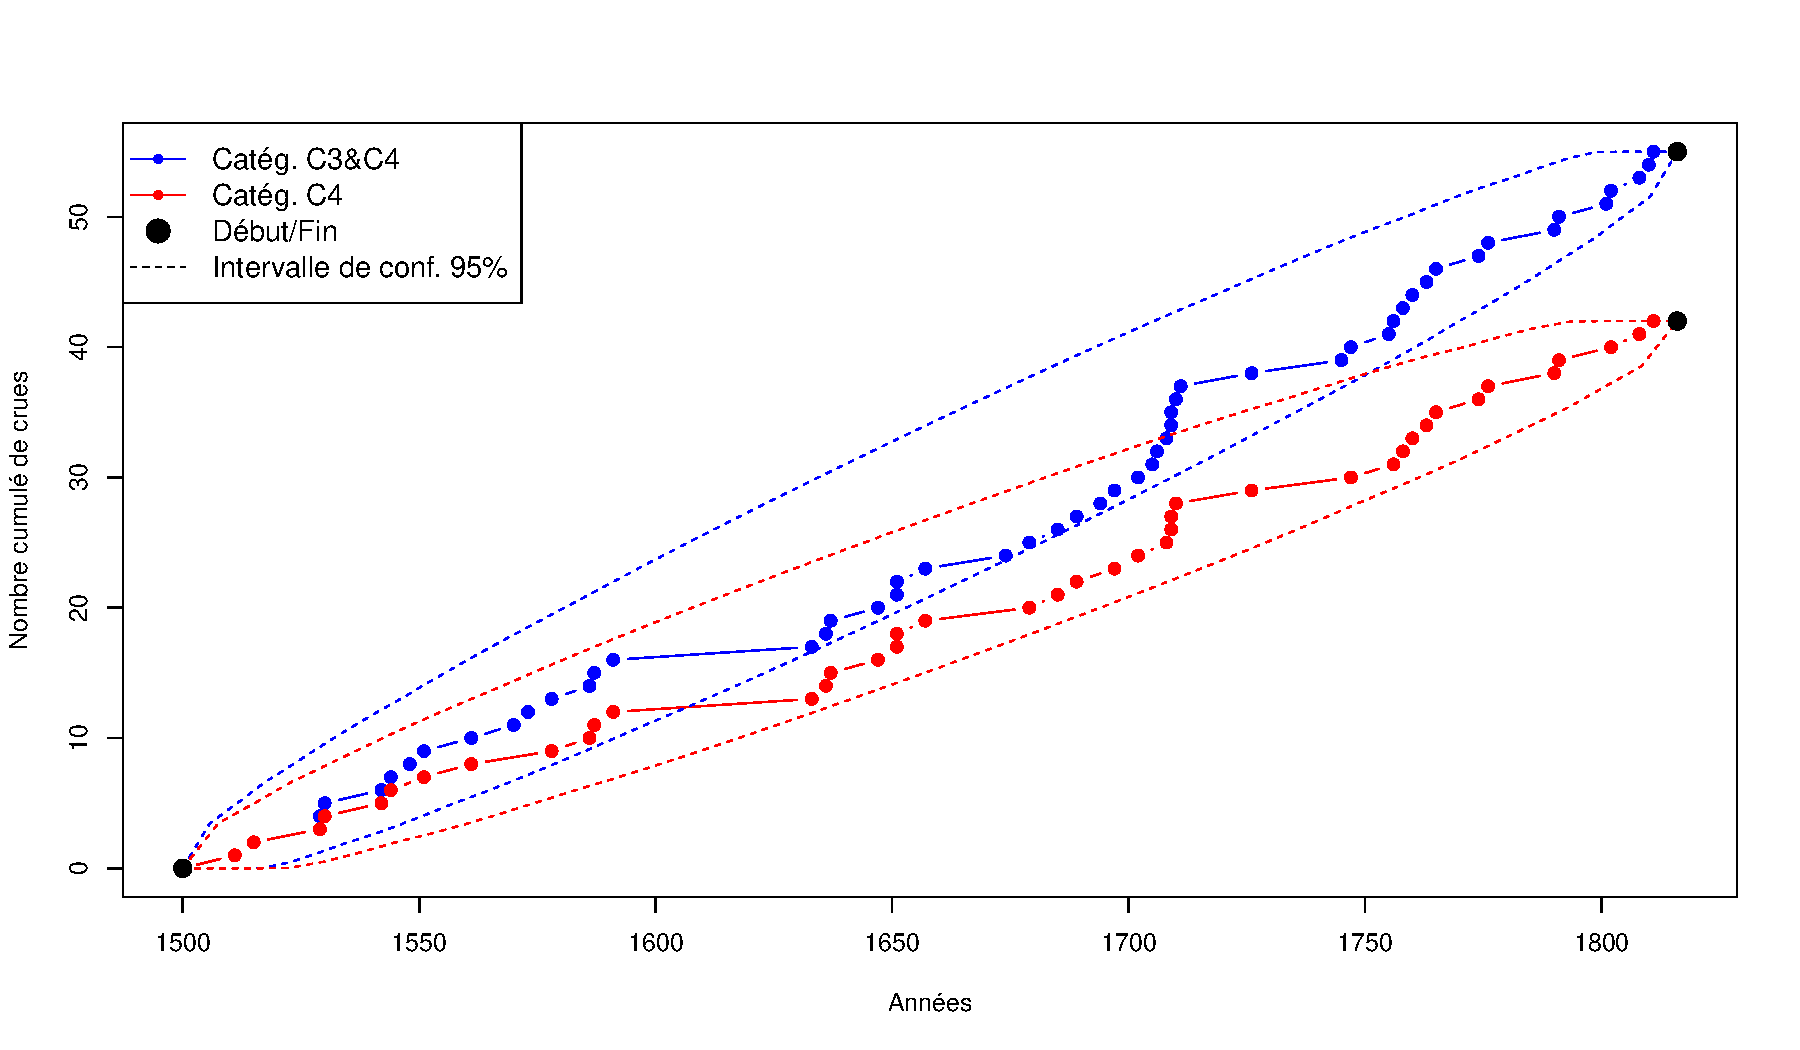
\includegraphics[width=.8\linewidth]{Chapitre4/Figures/Poisson_C3-C4_FR.pdf}	
		\caption{Nombre de crues cumulé et intervalles de confiance à 95\% du processus de 						Poisson, pour deux échantillons d'occurrences de crues supérieures aux seuils $S3$ (catégories C3 et C4) ou $S4$ (catégorie C4) à Beaucaire (1500-1816)}
		\label{fig:Poisson_C3-C4}
	\end{figure}		
	
	\paragraph{} Sur la figure \ref{fig:Poisson_C3-C4}, on remarque que les nombres cumulés de crues des deux échantillons sont compris dans les intervalles de confiance à 95\% des processus de Poisson, ils peuvent donc être tous deux considérés homogènes. L'échantillon correspondant au seuil $S3$ (en bleu) se rapproche de la borne inférieure de l'intervalle de confiance au XVII\textsuperscript{ème} siècle, mais revient rapidement dans des valeurs moyennes à la faveur de nombreuses crues supérieures au seuil au début du XVIII\textsuperscript{ème} siècle. 
	
	\paragraph{} L'échantillon continu de débits maximum annuels (1816-2020) sera par la suite artificiellement "dégradé" pour reproduire des durées de chroniques plus usuelles. Ainsi, les crues dont le débit maxpost est supérieur au seuil considéré sont retenues dans l'échantillon. Cette période "dégradée" commence au début de la chronique, en 1816, et se termine en 1970, à la mise en fonctionnement de la station de Beaucaire Restitution. Deux seuils de perception similaires aux seuils $S3$ et $S4$ sont ici étudiés : 7000 et 9000 $m^3/s$. L'homogénéité de ces deux échantillons "dégradés" est testée dans la figure \ref{fig:Poisson_Recent}. Les deux échantillons de crues cumulés sont compris dans les intervalles de confiance à 95\%, ils sont donc tous deux homogènes. 
	
	\begin{figure}[h]
		\centering
		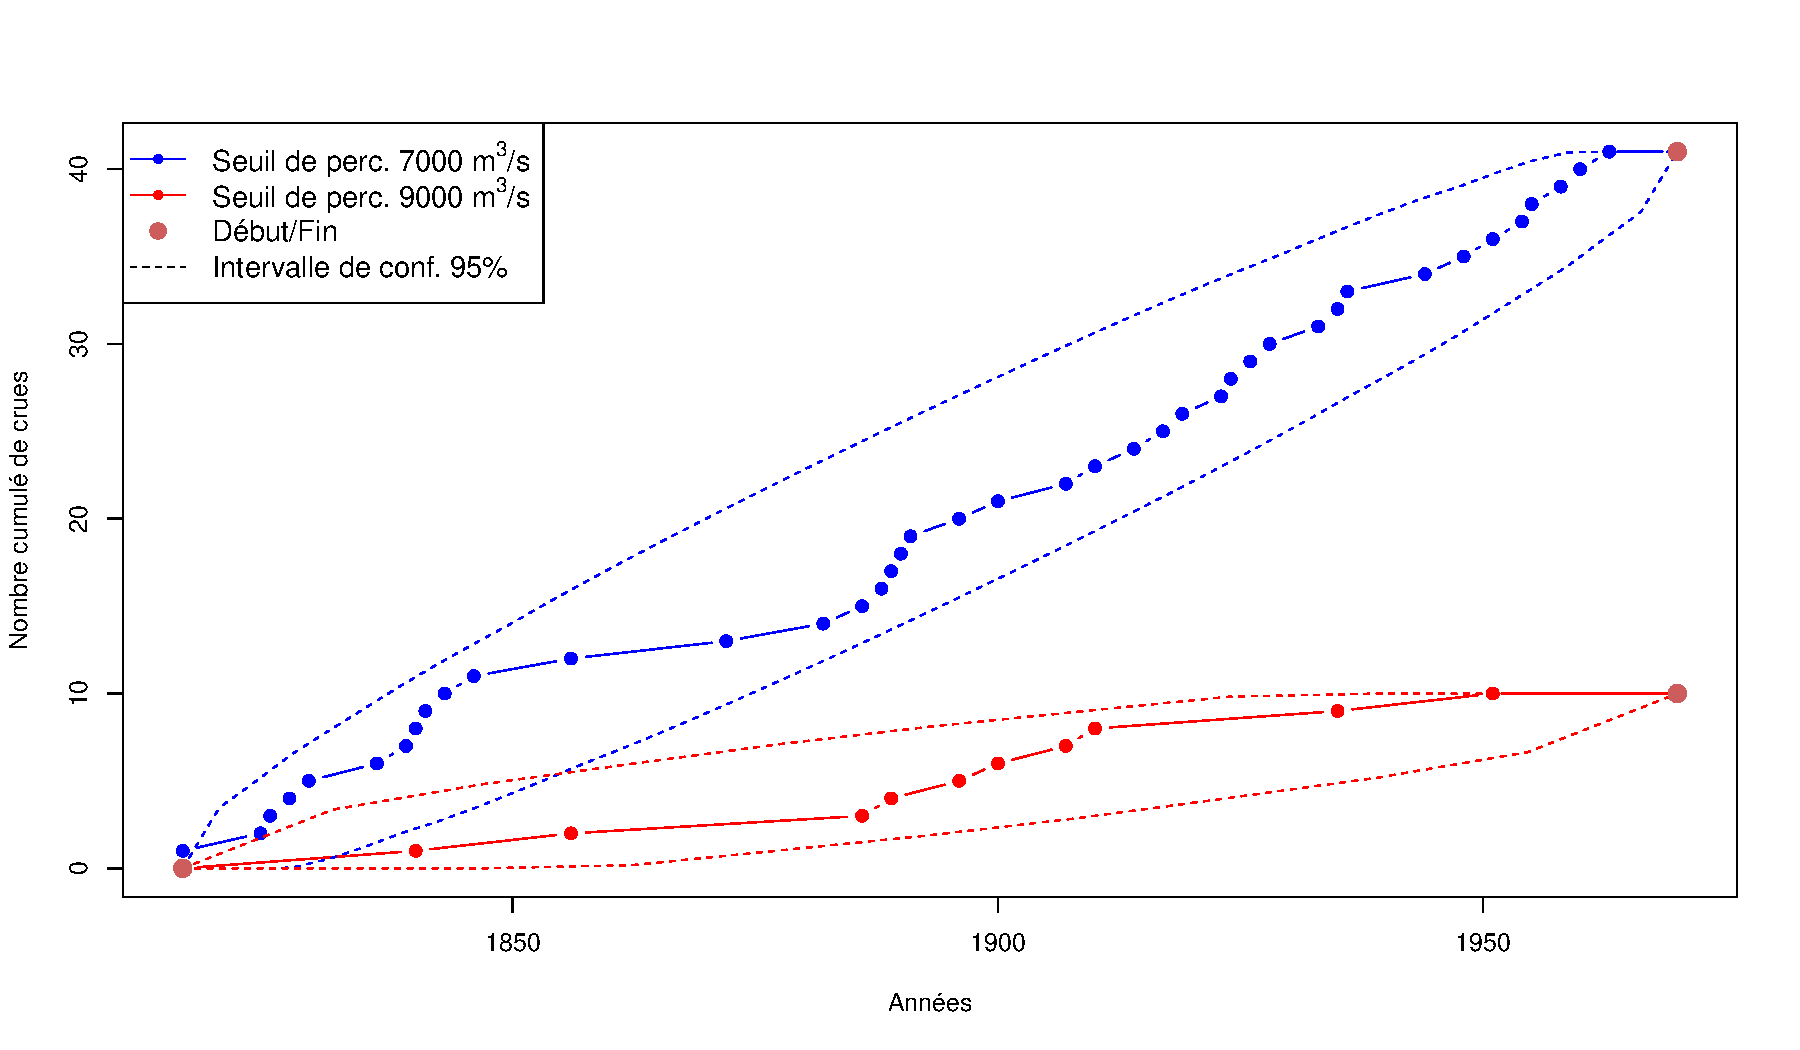
\includegraphics[width=.8\linewidth]{Chapitre4/Figures/Poisson_Qrecent_FR.pdf}	
		\caption{Nombre de crues cumulé et intervalles de confiance à 95\% du processus de 						Poisson, pour deux échantillons d'occurrences de crues supérieures aux seuils $S3$ ou $S4$ à Pont de Beaucaire 							(1816-1969) }
		\label{fig:Poisson_Recent}
	\end{figure}
	
	
	\paragraph{} Les échantillons de crues des périodes systématique et historique ont indépendamment été jugés homogènes. Il faut cependant garder à l'esprit que ces échantillons peuvent ne pas être homogènes entre eux pour diverses raisons. Par exemple, le seuil de perception utilisé pour l'échantillon systématique ($S3$ ou $S4$) peut ne pas être cohérent avec le seuil de perception de l'échantillon historique dont la valeur exacte est inconnue. 		
		
\FloatBarrier		
	
	
\section{Application aux crues du Rhône à Beaucaire}
\label{sec:applicationBcr}

	\paragraph{} Les 4 modèles décrits dans les sections précédentes (A, B, C et D) sont appliqués aux 4 échantillons de crues du Rhône à Beaucaire présentés dans le tableau \ref{tab:Echantillons}. Le modèle A fait l'hypothèse que le seuil de perception $S$ et la durée de la période historique $n$ sont parfaitement connus, tandis que dans le cas du modèle D, ces deux valeurs sont considérées incertaines. Le modèle B fait l'hypothèse que seul le seuil de perception $S$ est incertain, alors que pour le modèle C, seule la durée de la période historique $n$ est incertaine. Le modèle E suppose quant a lui que le débit des crues historique est connu et est contenu dans un intervalle d'incertitude, $S$ et $n$ sont alors supposés parfaitement connus. Pour les cinq modèles, l'incertitude des débits de la période continue est propagée. 
	
	\paragraph{} Les échantillons 1 et 2 représentent la combinaison des données pré-1816 décrites dans le chapitre \ref{chap:ch2} avec les données continues 1816-2020 estimées au chapitre \ref{chap:ch3}. Les échantillons 3 et 4 sont basés sur les débits estimés au chapitre \ref{chap:ch3} qui ont été dégradés pour créer artificiellement un échantillon mixte de données continues (1970-2020) et ponctuelles (1816-1969). Il s'agit ici de tailles d'échantillon plus usuelles et dont le seuil de perception et la durée de la période historique sont parfaitement connus, contrairement aux échantillons 1 et 2. Ainsi, pour les modèles faisant l'hypothèse que le seuil de perception et/ou la durée de la période historique sont inconnus, on jugera notamment la capacité du modèle à estimer des valeurs acceptables. 
	
	\begin{table}[h]
		\centering
		\caption{Caractéristiques des échantillons de crues du Rhône à Beaucaire. $S$ désigne le seuil de perception et $t^{*}$ la date de début de la période historique.}
		\label{tab:Echantillons}
		\resizebox{\columnwidth}{!}{%
		%\begin{tabular}{|l|l|l|l|ll|l|l|}
		\begin{tabular}{|c|c|c|c|cc|c|c|}
		\hline
		\multicolumn{1}{|c|}{\multirow{2}{*}{n°}} &
		  \multirow{2}{*}{Période historique} &
		  \multirow{2}{*}{Période continue} &
		  \multirow{2}{*}{Seuil $S$ [m\textsuperscript{3}/s]} &
		  \multicolumn{2}{c|}{Nb. de crues $> S$} &
		  \multirow{2}{*}{A priori $S$ [m\textsuperscript{3}/s]} &
		  \multirow{2}{*}{A priori $t^{*}$} \\ \cline{5-6}
		  
		 \multicolumn{1}{|c|}{} & & & & \multicolumn{1}{c|}{per. hist.} & per. cont. & & \\ \hline
		1 & 1500-1815 & 1816-2020 & 7000 & \multicolumn{1}{c|}{55} & 57 & $\mathcal{N}(7000,2000)$ & $\mathcal{U}(1111,1511)$ \\ \hline
		2 & 1500-1815 & 1816-2020 & 9000 & \multicolumn{1}{c|}{13} & 14 & $\mathcal{N}(9000,2000)$ & $\mathcal{U}(1129,1529)$ \\ \hline
		3 & 1816-1969 & 1970-2020 & 7000 & \multicolumn{1}{c|}{41} & 16 & $\mathcal{N}(7000,2000)$ & $\mathcal{U}(1316,1816)$ \\ \hline
		4 & 1816-1969 & 1970-2020 & 9000 & \multicolumn{1}{c|}{10} & 4 & $\mathcal{N}(9000,2000)$ & $\mathcal{U}(1340,1840)$ \\ \hline
		\end{tabular}%
		}
		
	\end{table}		
	
	Les modèles B, C et D font l'hypothèse que $S$ et/ou $n$ sont inconnus, il faudra donc affecter une distribution a priori à ces paramètres. Ces distributions sont présentées dans le tableau \ref{tab:Echantillons} pour chacun des échantillons. Le but étant ici d'explorer les performances des modèles, les a priori seront très peu informatifs. L'a priori du seuil de perception $S$ (modèles B et D) est supposé Gaussien, avec pour moyenne la valeur connue ou supposée du seuil (soit $S3$ ou $S4$) et pour écart type 2000 m\textsuperscript{3}/s. Par souci de clarté, on ne parlera pas ici de la durée de la période historique $n$ mais de la date de début de la période historique $t^{*}$ (la date de fin de la période historique étant ici parfaitement connue pour les 4 échantillons). La distribution a priori de $t^{*}$ (modèles C et D) est supposée uniforme avec pour borne supérieure la date de la première crue de l'échantillon historique considéré, appelée $t_{k=1}$. Par définition, la période historique débute au plus tard à la date de cette première crue. La borne inférieure de la distribution uniforme sera fixée 400 ans avant la date de la première crue $t_{k=1}$ afin de représenter la méconnaissance de $t^{*}$. 
			
	\FloatBarrier	
	
	\subsection{Résultats pour la période récente dégradée (1816-2020)}
	\label{subsec:ResultsArtif}
	
	\paragraph{} 
	Les 4 modèles décrits dans la section \ref{sec:MethodoCh3} ont été appliqués à l'échantillon 4 du tableau \ref{tab:Echantillons}. Les estimations pour les crues centennales et millénales sont présentées dans la figure \ref{fig:Barplot_Artif2}, dans laquelle les 4 modèles GEV-Binomiale sont comparés au modèle GEV (chapitre \ref{chap:ch3}) appliqué successivement à la chronique continue totale (1816-2020) et à la chronique continue dégradée (1970-2020). Ces mêmes résultats sont détaillés dans le tableau \ref{tab:ResArtif2}, où la valeur des paramètres est présentée. Enfin, la figure \ref{fig:Quantiles_Artif2} présente l'ensemble des quantiles jusqu'à la crue décamillénale pour les 6 modèles. On peut ici juger l'adéquation des quantiles avec les observations. Le rang des crues supérieures au seuil est tiré aléatoirement comme décrit dans la section \ref{subsec:DistEmpirique}. 	
	
	\begin{figure}[h]
		\centering
		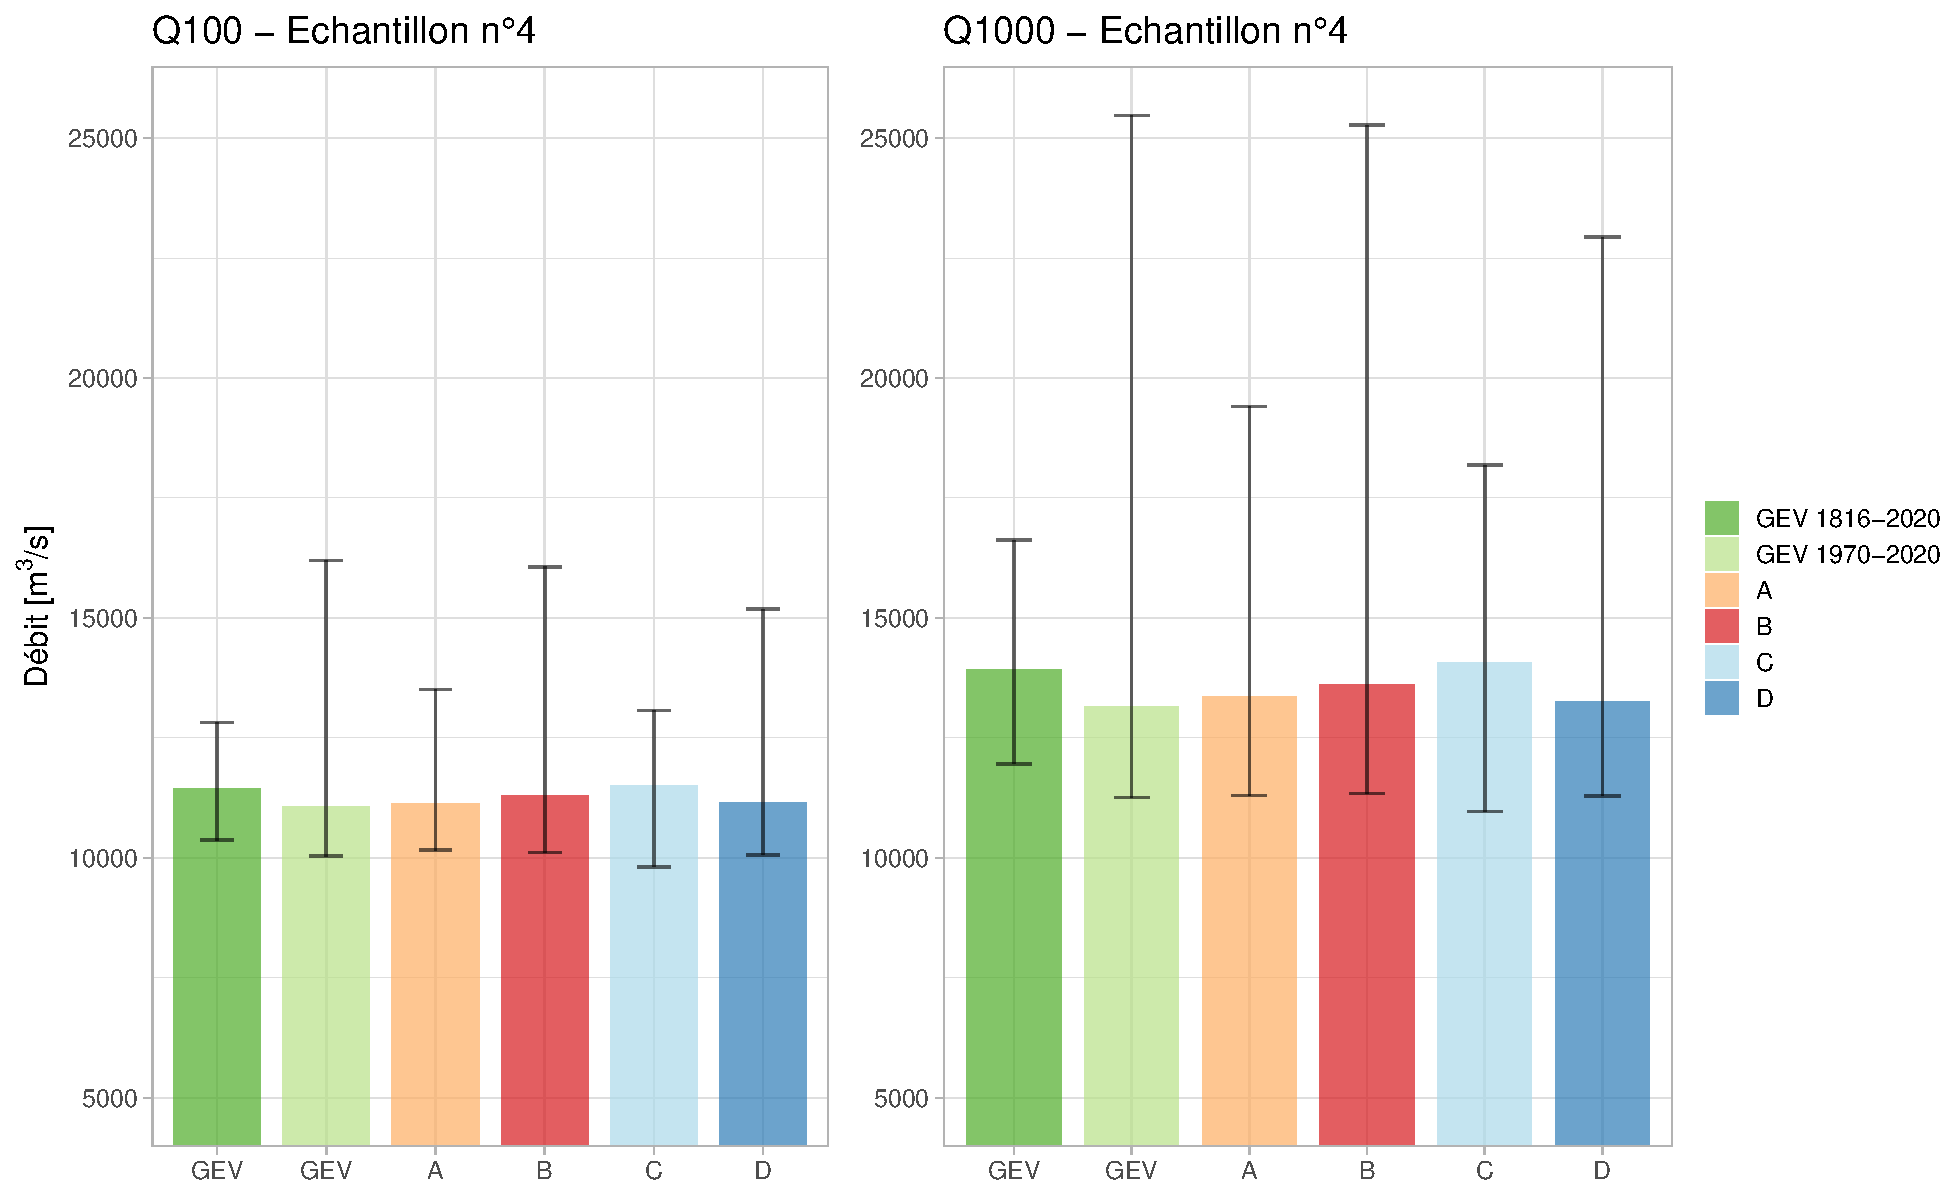
\includegraphics[width=.8\linewidth]{Chapitre4/Figures/Barplots_QX_Artif2.pdf}	
		\caption{Estimations maxpost et incertitudes à 95\% pour Q100 et Q1000 pour 6 modèles appliqués à l'échantillon 4 (1816-2020 dégradé, $S4$)}
		\label{fig:Barplot_Artif2}
	\end{figure}

	\begin{table}[h]
	\centering
	\caption{Résultats maxpost et incertitudes des 7 modèles appliqués à l'échantillon 4. Q100 et Q1000 représentent respectivement le débit des crues centennales et millénales, $\xi$ le paramètre de forme de la distribution GEV, $S$ le seuil de perception et $t^{*}$ la date de début de la période historique. Les écarts type des distributions a posteriori sont représentés par les colonnes débutant par la lettre "u". \textcolor{red}{DEPLACER PLUS PROCHE DE LA PARTIE MODELE E?} }
	\label{tab:ResArtif2}
	\resizebox{\columnwidth}{!}{%
		\begin{tabular}{|c|c|c|c|c|c|c|c|c|c|c|}
		\hline
Modèle & Q100 [m\textsuperscript{3}/s] & uQ100 [m\textsuperscript{3}/s] & Q1000 [m\textsuperscript{3}/s] & uQ1000 [m\textsuperscript{3}/s] & $\xi$ & $u\xi$ & $S$ [m\textsuperscript{3}/s] & $uS$ [m\textsuperscript{3}/s] & $t^{*}$ & $ut^{*}$ \\ \hline
GEV 1816-2020 & 11451 & 687   & 13919 & 1351   & 0.058 & 0.044  & X    & X    & X    & X  \\ \hline
GEV 1970-2020 & 11076 & 2560  & 13154 & 6159   & 0.077 & 0.102  & X    & X    & X    & X  \\ \hline
A             & 11132 & 1189  & 13367 & 3019   & 0.062 & 0.088  & 9000 & X    & 1816 & X  \\ \hline
B             & 11302 & 2381  & 13622 & 5823   & 0.058 & 0.102  & 9163 & 729  & 1816 & X  \\ \hline
C             & 11517 & 779   & 14069 & 2057   & 0.041 & 0.083  & 9000 & X    & 1833 & 71 \\ \hline
D             & 11147 & 2018  & 13262 & 4837   & 0.074 & 0.096  & 9332 & 883  & 1785 & 107 \\ \hline
E       	  & 11286 & 932   & 13827 & 2255   & 0.039 & \textcolor{red}{??} &  9000 & X & 1816 & X \\ \hline
		\end{tabular}}

	\end{table}

	\begin{figure}[h]
		\centering
		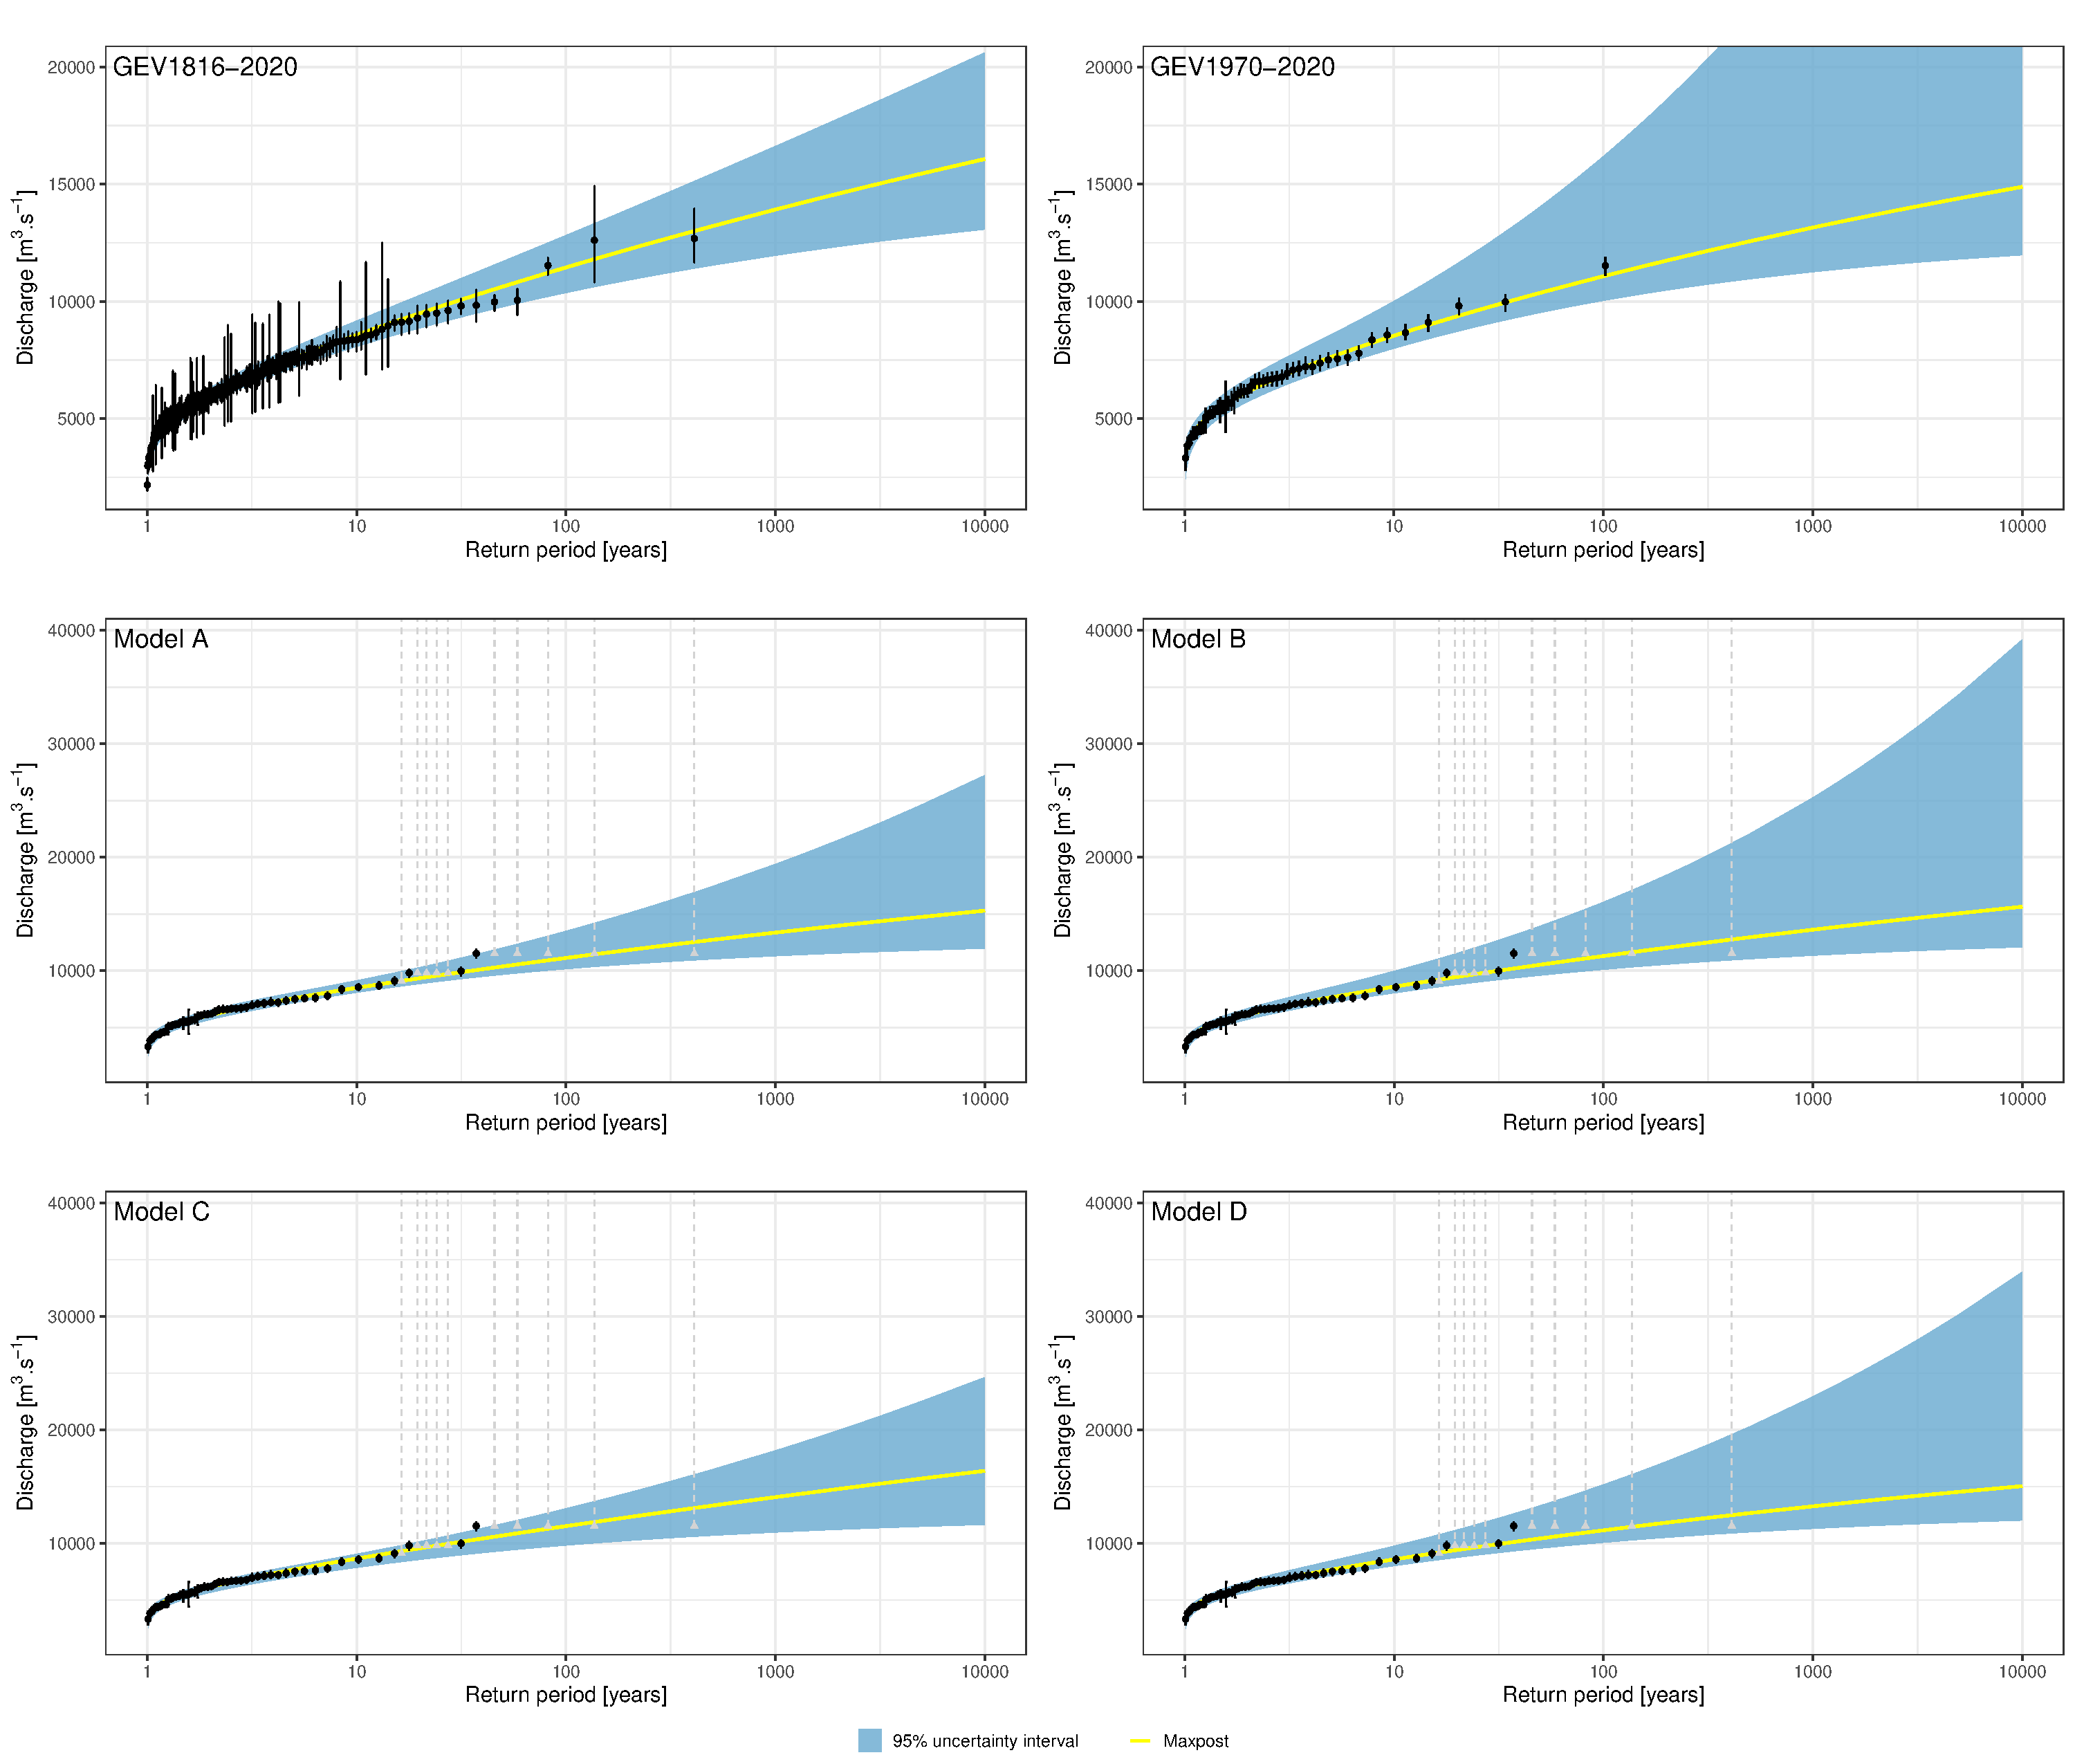
\includegraphics[width=\linewidth]{Chapitre4/Figures/Quantiles_Artif2.pdf}	
		\caption{Quantiles de débit maximum annuel estimés par 6 modèles pour l'échantillon 4 (1816-2020 dégradé, $S4$). Les observations sont en noir pour la période continue (l'incertitude est également représentée) et en gris pour la période historique.}
		\label{fig:Quantiles_Artif2}
	\end{figure}
	

\FloatBarrier
	
	\subsubsection{Quel est l'apport de l'utilisation des crues historiques pour une longueur de chronique "courante" ?}
	
	\paragraph{} Une durée de chronique continue trop courte devant la période de retour du quantile visé entraîne des résultats très incertains (GEV 1970-2020 dans les figures \ref{fig:Barplot_Artif2} et \ref{fig:Quantiles_Artif2}). La durée de la chronique continue (50 ans) est ici très petite devant la période de retour visée (100 ou 1000 ans). Si on se trouve dans l'impossibilité de reconstituer des débits en continu au-delà de 50 ans, on remarque que l'utilisation d'occurrences de crues historiques permet de réduire l'incertitude (modèle A en orange). Évidemment, l'utilisation d'occurrences de crues ne permet pas d'atteindre la précision obtenue avec 200 ans de chronique continue (GEV 1816-2020 en vert foncé), mais l'incertitude obtenue s'en rapproche en utilisant les crues historiques, tout particulièrement lorsque $S$ et $n$ sont connus. En revanche, les estimations maxpost de l'ensemble des modèles sont proches. 
	
	\paragraph{} Pour les 6 modèles, une part de l'incertitude provient de l'estimation du paramètre de forme qui gouverne le comportement de la queue de distribution. On retrouve les valeurs a posteriori du paramètre de forme dans la figure \ref{fig:Shape_Artif2}. On notera que l'ensemble des estimations sont proches de zéro et légèrement positives, on se trouve donc dans le cas "queue légère" de la distribution GEV (cas "loi de Weibull"). Comme l'on peut s'y attendre, l'estimation de ce paramètre est plus précise dans le cas GEV 1816-2020. Les distributions a posteriori sont très proches pour les modèles A et C (tableau \ref{tab:ResArtif2}). 
	
	\textcolor{red}{
	\paragraph{RMQ BEN} D'ailleurs comme on ne réduit que faiblement l'incertitude sur xi par rapport à GEV 1970-2020, d'où vient la réduction d'incertitude des quantiles? De position et échelle j'imagine? Comme tu as de la place en figure 6 est-ce que ca ne vaudrait pas le coup de mettre les 3 paramètres? A FAIRE S'IL RESTE DU TEMPS
	}
	
	\begin{figure}[h]
		\centering
		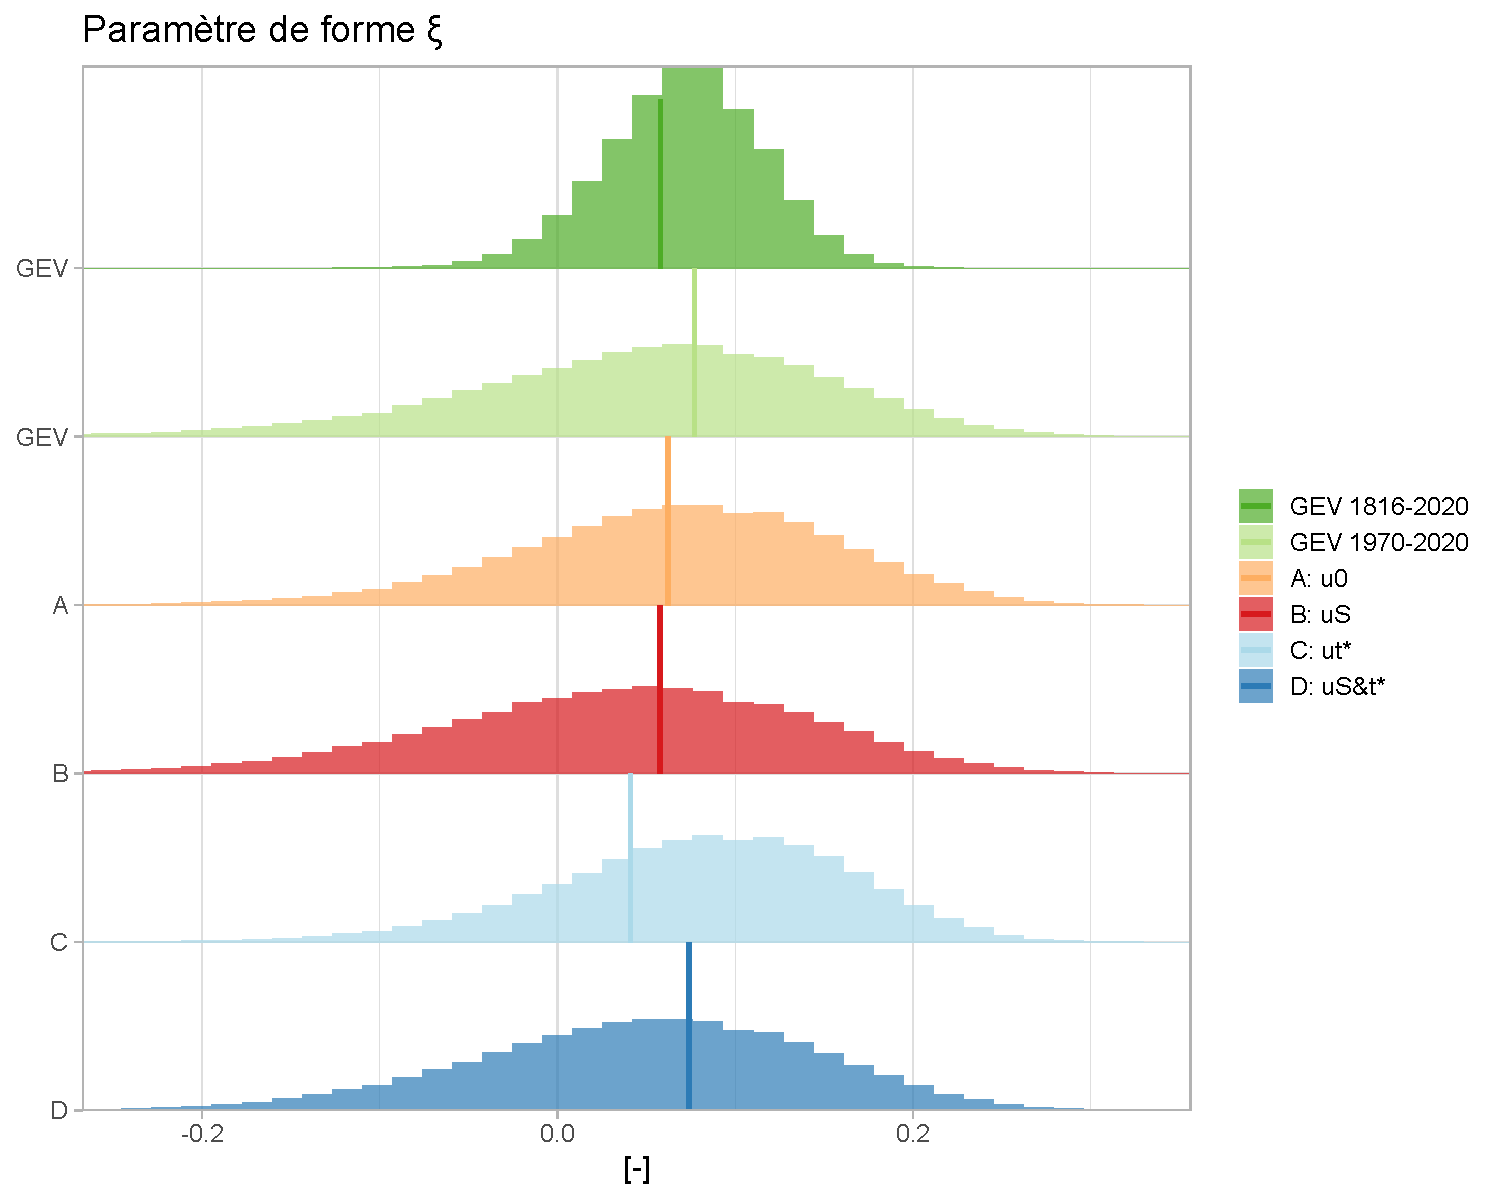
\includegraphics[width=.6\linewidth]{Chapitre4/Figures/Shape_Artif2.pdf}	
		\caption{Distributions a posteriori du paramètre de forme de la distribution GEV des débits maximum annuels pour les 4 modèles estimés sur l'échantillon 4. Les estimations des modèles GEV sont également indiquées. Les droites verticales représentent les valeurs maxpost.}
		\label{fig:Shape_Artif2}
	\end{figure}

\FloatBarrier
	
	\subsubsection{Quel est l'impact de la méconnaissance du seuil de perception sur l'estimation des quantiles ?}
	
	\paragraph{} L'utilisation du modèle B reflète la méconnaissance du seuil de perception, celui-ci devenant alors un paramètre à part entière du modèle. Sur la figure \ref{fig:Barplot_Artif2}, on constate que l'incertitude autour des quantiles estimés par le modèle B est bien plus importante que pour le modèle A, et se rapproche de celle obtenue avec les données continues seulement (GEV 1970-2020). La méconnaissance du seuil a donc des conséquences importantes sur les estimations puisqu'elle réduit fortement l'intérêt d'utiliser les occurrences historiques. La vraie valeur du seuil de perception pour l'échantillon 4 est $S4$ = 9000 m\textsuperscript{3}/s. On retrouve les distributions a priori et a posteriori du seuil dans la figure \ref{fig:Params_Artif2}. On remarque que l'a posteriori pour le modèle B est proche de la vraie valeur, et que le modèle a effectivement permis d'améliorer la connaissance du seuil par rapport à l'a priori renseigné qui est ici très incertain : $\mathcal{N}(9000,2000)$. La valeur maxpost est de 9163 m\textsuperscript{3}/s soit une erreur relative de 2\%. Dans une situation plus réaliste, un a priori du seuil de perception plus précis aurait pu être choisi afin de limiter cet impact. Il faut également noter que l'incertitude a posteriori du paramètre de forme pour le modèle B (figure \ref{fig:Shape_Artif2}) est plus grande que celle du modèle A et devient alors quasi-identique à celle du modèle GEV 1970-2020. 
	
	 \begin{figure}[h]
		\centering
		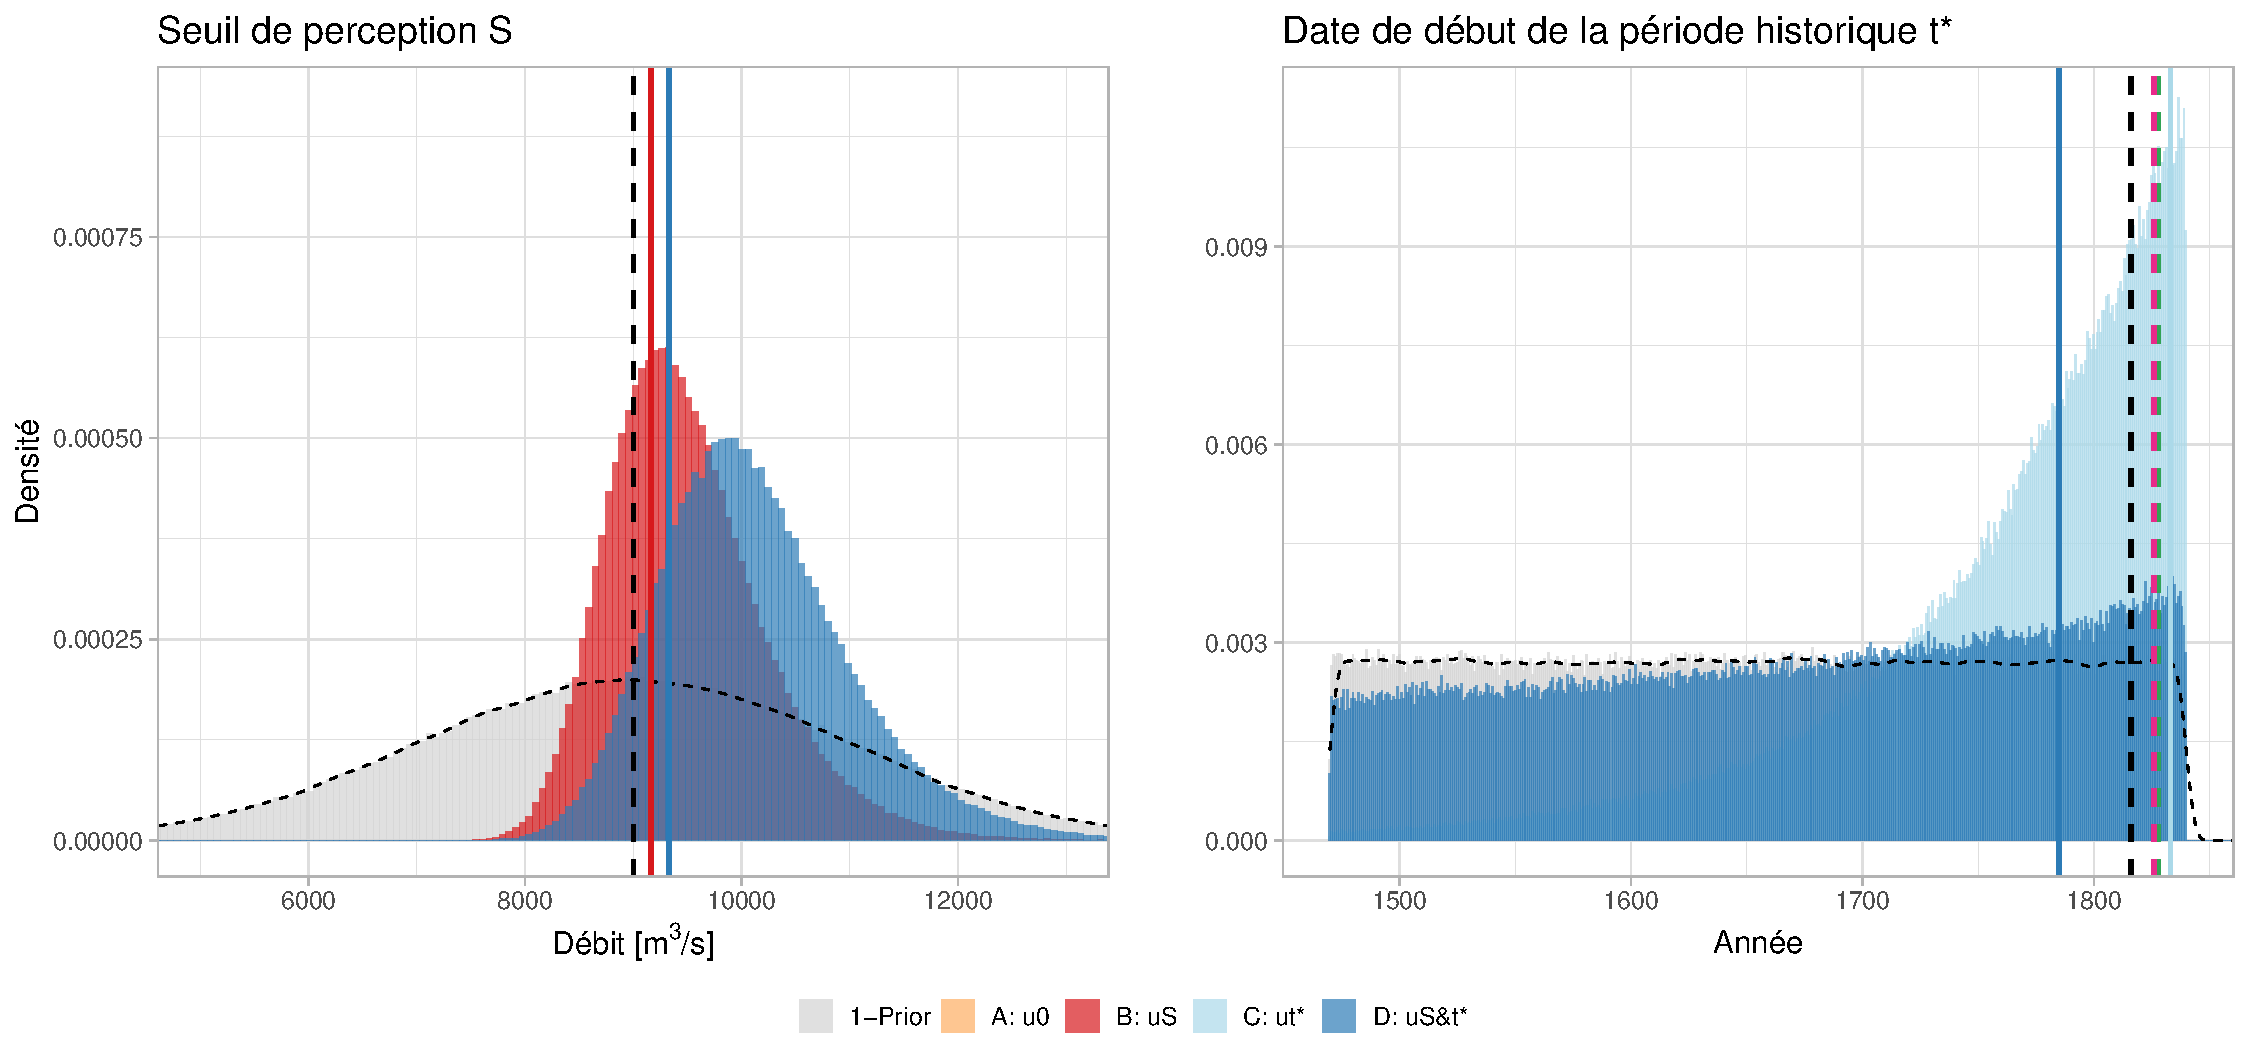
\includegraphics[width=.9\linewidth]{Chapitre4/Figures/Params_Artif2.pdf}	
		\caption{Distributions a priori et a posteriori pour le seuil de perception (gauche) et la date de début de la période historique (droite). Les droites verticales pleines représentent l'estimation maxpost du paramètre pour chacun des modèles et les droites en pointillés noirs représentent les valeurs de référence. Les droites verticales en pointillés vert et rose représentent respectivement les estimations de $t^{*}$ par la méthode de \citet{prosdocimi_german_2018} et la méthode de la période de retour du seuil $S$.}
		\label{fig:Params_Artif2}
	\end{figure}
	
	\subsubsection{Quel est l'impact de la méconnaissance de la durée de la période historique sur l'estimation des quantiles ?}	
	
	\paragraph{} Le modèle C permet de représenter la méconnaissance de la durée de la période historique, qui est l'un des deux paramètres de la loi binomiale utilisée ici pour modéliser le nombre d'occurrences de crues supérieures à un seuil. Sur la figure \ref{fig:Barplot_Artif2}, les estimations maxpost des quantiles pour le modèle C ont des valeurs légèrement supérieures aux estimations du modèle A. Cette légère sur-estimation provient d'une durée de période historique sous-estimée par le modèle, visible sur la figure \ref{fig:Params_Artif2} (droite). En effet, la date maxpost est l'année 1833, alors que la chronique débute réellement en 1816. Cette sous-estimation de 16 ans peut s'expliquer par une fréquence des crues supérieures au seuil $S4$ plus importante au cours de la période continue (4 crues / 50 ans = 0.08 crues/an) qu'au cours de la période historique (10 crues / 153 ans = 0.065 crues/an). Ce déséquilibre reflète l'existence d'oscillations dans la fréquence d'occurrence des crues dues à la variabilité d'échantillonnage, malgré le fait qu'aucune non-stationnarité des données n'ait été détectée par les tests à la section \ref{subsec:homog}. Il faut également noter que la distribution a posteriori pour le modèle C (figure \ref{fig:Params_Artif2}, droite) est largement réduite par rapport à l'a priori, et présente une forme très asymétrique. La distribution connait un maximum entre 1820 et 1840. Même si la valeur maxpost de $t^*$ est relativement éloignée de la vraie valeur (17 ans), la distribution a posteriori converge vers des valeurs cohérentes par rapport à l'a priori très peu informatif qui a été donné. 	 
	
	\paragraph{} L'incertitude autour des quantiles estimée par le modèle C est très similaire à celle estimée par le modèle A (figure \ref{fig:Barplot_Artif2}), de même que la distribution du paramètre de forme (figure \ref{fig:Shape_Artif2}). Une forte méconnaissance de la durée de la période historique n'a donc que peu d'impact sur la précision de l'estimation des quantiles, contrairement à la méconnaissance du seuil de perception.
	
	\subsubsection{Quel est l'impact de la méconnaissance du seuil de perception et de la durée de la période historique sur l'estimation des quantiles ?}	
	
	\paragraph{} Représenter la méconnaissance autour de $S$ et $n$ en même temps dans le modèle probabiliste paraît être la solution la plus raisonnable dans certains cas, notamment pour des événements très anciens et mal connus. Le modèle D est ici utilisé à cet effet. Les quantiles maxpost estimés dans la figure \ref{fig:Barplot_Artif2} pour le modèle D semblent cohérents avec les valeurs de référence. En revanche, la largeur de l'intervalle de confiance est importante et se situe entre celle du modèle B et du modèle C. Même si l'estimation est plus précise que celle du modèle GEV sur l'échantillon 1970-2020, elle reste imprécise pour la crue millénale. L'observation des paramètres a posteriori sur la figure \ref{fig:Params_Artif2} permet de comprendre l'origine de cette large incertitude. La distribution du seuil de perception, bien que centrée a proximité de la vraie valeur (maxpost à 9331 m\textsuperscript{3}/s), est très large (écart type = 883 m\textsuperscript{3}/s). Le seuil de perception parait ici un peu moins bien estimé que par le modèle B (écart type = 729 m\textsuperscript{3}/s). La date de début de la période historique est elle encore plus difficilement estimée, notamment en comparaison avec l'estimation du modèle C. On remarque que la distribution a posteriori est très similaire à celle de l'a priori, même si elle est légèrement asymétrique et marque un maximum non loin de la vraie valeur (l'année 1816). Cependant, les quantiles présentent une plus faible incertitude pour le modèle D que pour le modèle B. Cela provient de corrélations entre les paramètres qui peuvent être observées sur la figure \ref{fig:ScatterD_Artif2}. On remarque notamment une assez bonne corrélation entre la durée de la période historique $n$ et le seuil de perception $S$, ainsi qu'entre le seuil de perception et le paramètre de forme $\xi$. Il est donc complexe d'identifier ces paramètres séparément. Une élicitation plus précise de leurs a priori sera certainement nécessaire.
	
	\begin{figure}[h]
		\centering
		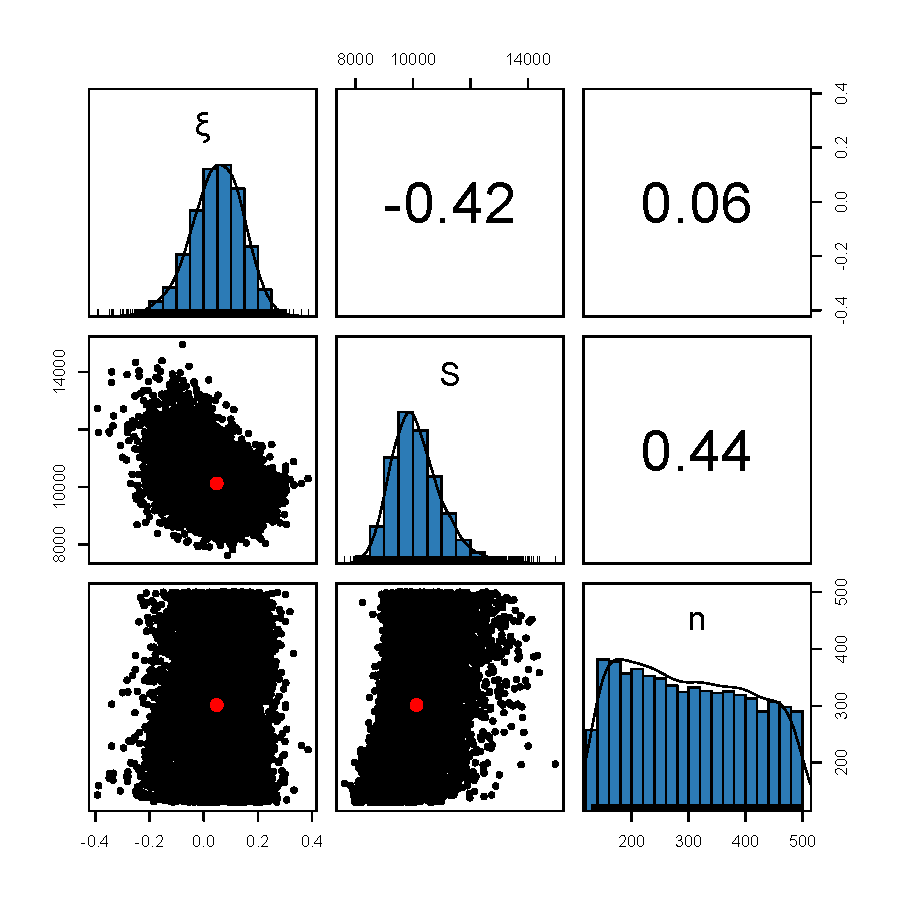
\includegraphics[width=.7\linewidth]{Chapitre4/Figures/ScatterD_Artif2.pdf}
		\caption{Scatterplots des distributions a posteriori de trois paramètres du modèle D pour l'échantillon 4 : le paramètre de forme $\xi$ (sans unité), le seuil de perception $S$ (en m\textsuperscript{3}/s) et la durée de la période historique $n$ (en années). Les nombres inscrits dans les cases supérieures correspondent aux corrélations entre les paramètres et les points rouges correspondent aux médianes.}
		\label{fig:ScatterD_Artif2}
	\end{figure}
		
\FloatBarrier

	\subsubsection{Quel est l'apport de la connaissance du débit des crues historiques ?}

	\paragraph{} Les modèles A, B, C et D n'utilisent que l'information du nombre de dépassements $k$ d'un seuil de perception $S$ pendant une durée $n$. Le débit des crues historiques ayant dépassé le seuil est donc ignoré. Le modèle E permet de prendre en compte cette donnée de débit ainsi que l'incertitude correspondant à chaque crue. Il a été appliqué à l'échantillon 4 du tableau \ref{tab:Echantillons} en considérant l'incertitude des débits de la période historique (1816-1969) calculée au chapitre \ref{chap:ch3}.
	
	
	\begin{figure}[h]
		\centering
		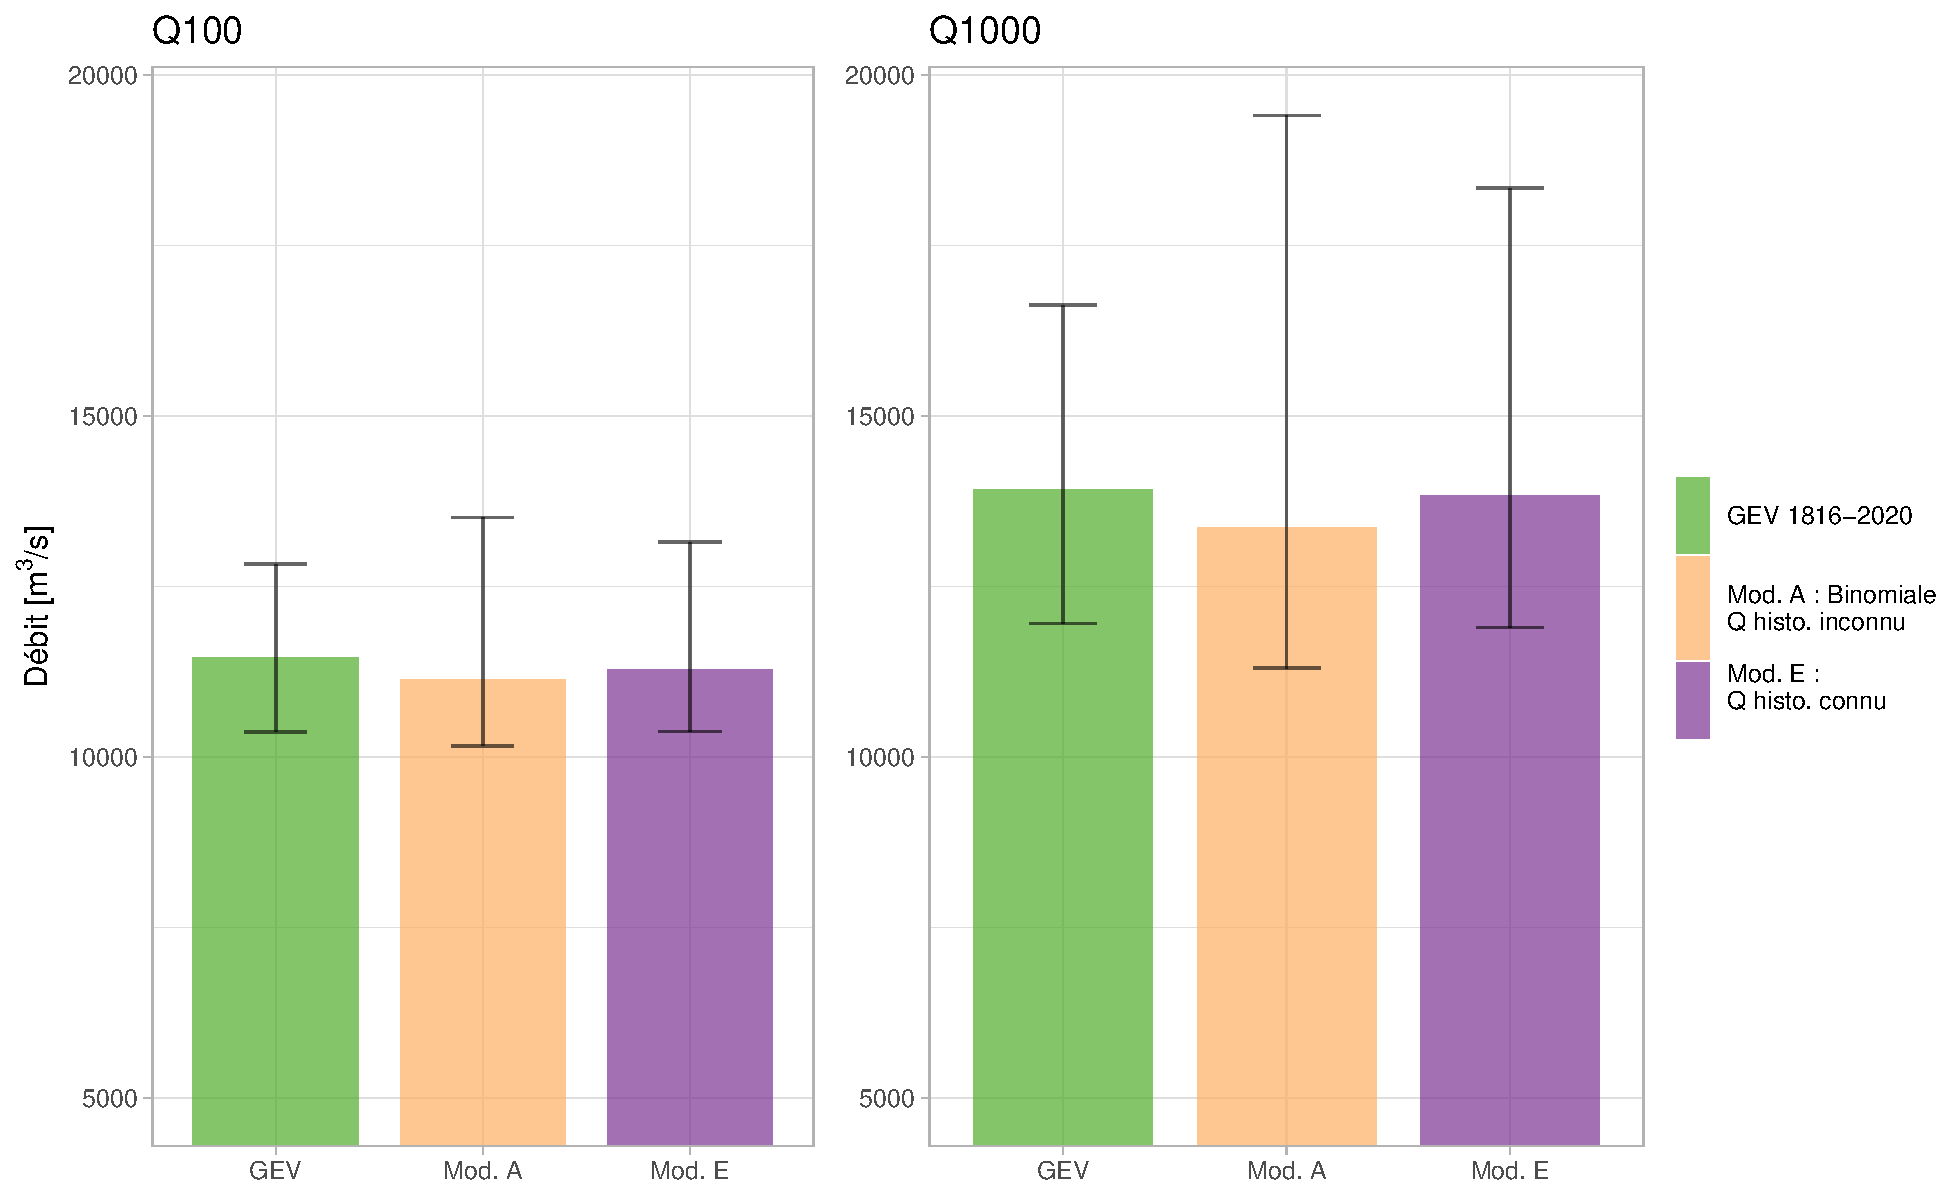
\includegraphics[width=.8\linewidth]{Chapitre4/Figures/Barplots_QX_censure.pdf}
		\caption{Estimations maxpost et incertitudes à 95\% pour Q100 et Q1000 pour 3 modèles appliqués à l'échantillon 4 (1816-2020 dégradé, $S4$). Le modèle A n'utilise que le nombre de dépassements du seuil de perception, alors que le modèle E considère le débit des crues historiques (et son incertitude) ayant dépassé le seuil $S$.}
		\label{fig:CensureArtif}
	\end{figure}
	
%	\begin{table}[h]
%		\centering
%		\caption{Résultats maxpost et incertitudes pour trois modèles appliqués à l'échantillon 4. Q100 et Q1000 représentent respectivement le débit des crues centennales et millénales. Les écarts type des distributions a posteriori sont représentés par les colonnes débutant par la lettre "u". \textcolor{red}{A BASCULER DANS LE TABLEAU 2}}
%		\label{tab:ResCensure}
%%		\resizebox{\columnwidth}{!}{%
%		\begin{tabular}{|c|c|c|c|c|}
%			\hline
%			Modèle        & Q100 [m\textsuperscript{3}/s] & uQ100 [m\textsuperscript{3}/s] & Q1000 [m\textsuperscript{3}/s] & uQ1000 [m\textsuperscript{3}/s] \\ \hline
%			GEV 1816-2020 & 11451 & 687   & 13919 & 1351   \\ \hline
%			A             & 11132 & 1189  & 13367 & 3019   \\ \hline
%			E       & 11286 & 932   & 13827 & 2255   \\ \hline
%		\end{tabular}%}
%		
%	\end{table}
%	
	\paragraph{}
	Les résultats sont présentés dans la figure \ref{fig:CensureArtif} et le tableau \ref{tab:ResArtif2}. On constate une diminution de l'incertitude d'environ 25\% autour du Q1000 pour le modèle E (avec un écart type de 2255 [m\textsuperscript{3}/s] pour Q1000) par rapport au modèle binomial A (écart type de 3019 [m\textsuperscript{3}/s] pour Q1000). En revanche, l'incertitude du modèle E reste environ 65\% supérieure à celle du modèle GEV 1816-2020 pour Q1000. La connaissance du débit des crues historiques, bien qu'elle ne soit pas une condition nécessaire à l'utilisation de données pré-enregistrements systématiques, permet donc de réduire l'incertitude autour des quantiles extrêmes. Cette incertitude reste en revanche supérieure à celle du modèle GEV pour lequel le débit maximum annuel de toutes les années de l'échantillon (historique + continu) est connu.	

	\subsubsection{Discussion intermédiaire}
	
	\paragraph{} L'utilisation des modèles décrits dans la section \ref{sec:MethodoCh3} sur un échantillon artificiellement dégradé et dont les caractéristiques sont parfaitement connues permet d'évaluer la performance des modèles et l'impact de la méconnaissance du seuil de perception $S$ et de la durée de la période historique $n$ sur l'estimation des quantiles extrêmes. On constate en observant les résultats que la méconnaissance du seuil de perception a un plus fort impact sur l'incertitude des résultats que la méconnaissance de la durée de la période historique. Même si les distributions a posteriori du seuil de perception pour les modèles B et D sont centrées a proximité de la vraie valeur (9000 m\textsuperscript{3}/s), l'incertitude résultant de la détermination du seuil a un fort impact sur l'incertitude des quantiles. En revanche, l'estimation de la durée de la période historique dans le cas des modèles C et D semble elle aussi relativement peu précise, mais n'impacte que peu l'incertitude des résultats si on compare ces derniers à ceux du modèle A. Cela est dû à des corrélations entre paramètres (figure \ref{fig:ScatterD_Artif2}) qui entraînent une réduction de l'incertitude finale.
	 
	\paragraph{} Ces premiers résultats démontrent que l'incertitude des quantiles peut être sous-estimée	lorsque l'on considère seuil de perception et durée de période historique comme étant bien connus alors que ce n'est pas le cas. Les modèles utilisés ici permettent de prendre en compte cette méconnaissance dans l'estimation des quantiles extrêmes. On pourra par la suite les appliquer au cas réel de l'échantillon de crues de la période 1500-2020 à Beaucaire, dont le seuil de perception et la durée de période historique ne sont pas connus précisément. Si les a priori utilisés jusqu'ici étaient peu informatifs afin de comprendre les performances du modèle, ils devront être élicités plus précisément par la suite afin d'obtenir des résultats qui reflètent davantage la connaissance/méconnaissance du seuil de perception et de la durée de la période historique.
		
	\paragraph{} Enfin, la comparaison du modèle A pour lequel seul le nombre de dépassements du seuil de perception est connu avec le modèle E pour lequel le débit des crues historiques est connu (ainsi que l'incertitude autour de ces débits) a permis de démontrer l'intérêt de reconstituer le débit des crues historiques. Néanmoins, ces résultats ne sont valables que pour le seuil de perception $S4$ utilisé ici. Plusieurs études (notamment \citet{stedinger_flood_1986} et \citet{payrastre_usefulness_2011}) ont démontré que l'écart d'incertitude entre les résultats de ces deux types de modèles tendait à se réduire à mesure que la période de retour du seuil de perception tendait vers environ 50 ans, jusqu'à devenir nul au delà de cette magnitude. Cela encourage donc l'utilisation du nombre de dépassements d'un seuil de perception lorsqu'il n'est pas possible d'avoir de meilleure information sur la période historique.
	
	\subsection{Application à la période 1500-2020}
	\label{subsec:Results1500}
	
	\paragraph{} Les modèles A, B, C et D de la section \ref{sec:MethodoCh3} ont été appliqués à l'échantillon 2 (1500-2020, seuil $S4$). Les estimations centennales et millénales sont présentés dans la figure \ref{fig:BarplotC4} et sont comparés au modèle GEV sur l'échantillon continu 1816-2020. On retrouve également ces résultats dans le tableau \ref{tab:ResC4}, accompagnés des valeurs a posteriori de certains paramètres du modèle. Les distributions a posteriori de $S$ et $t^{*}$ sont également représentées dans la figure \ref{fig:Params_C4}.
	
	
	\begin{figure}[h]
		\centering
		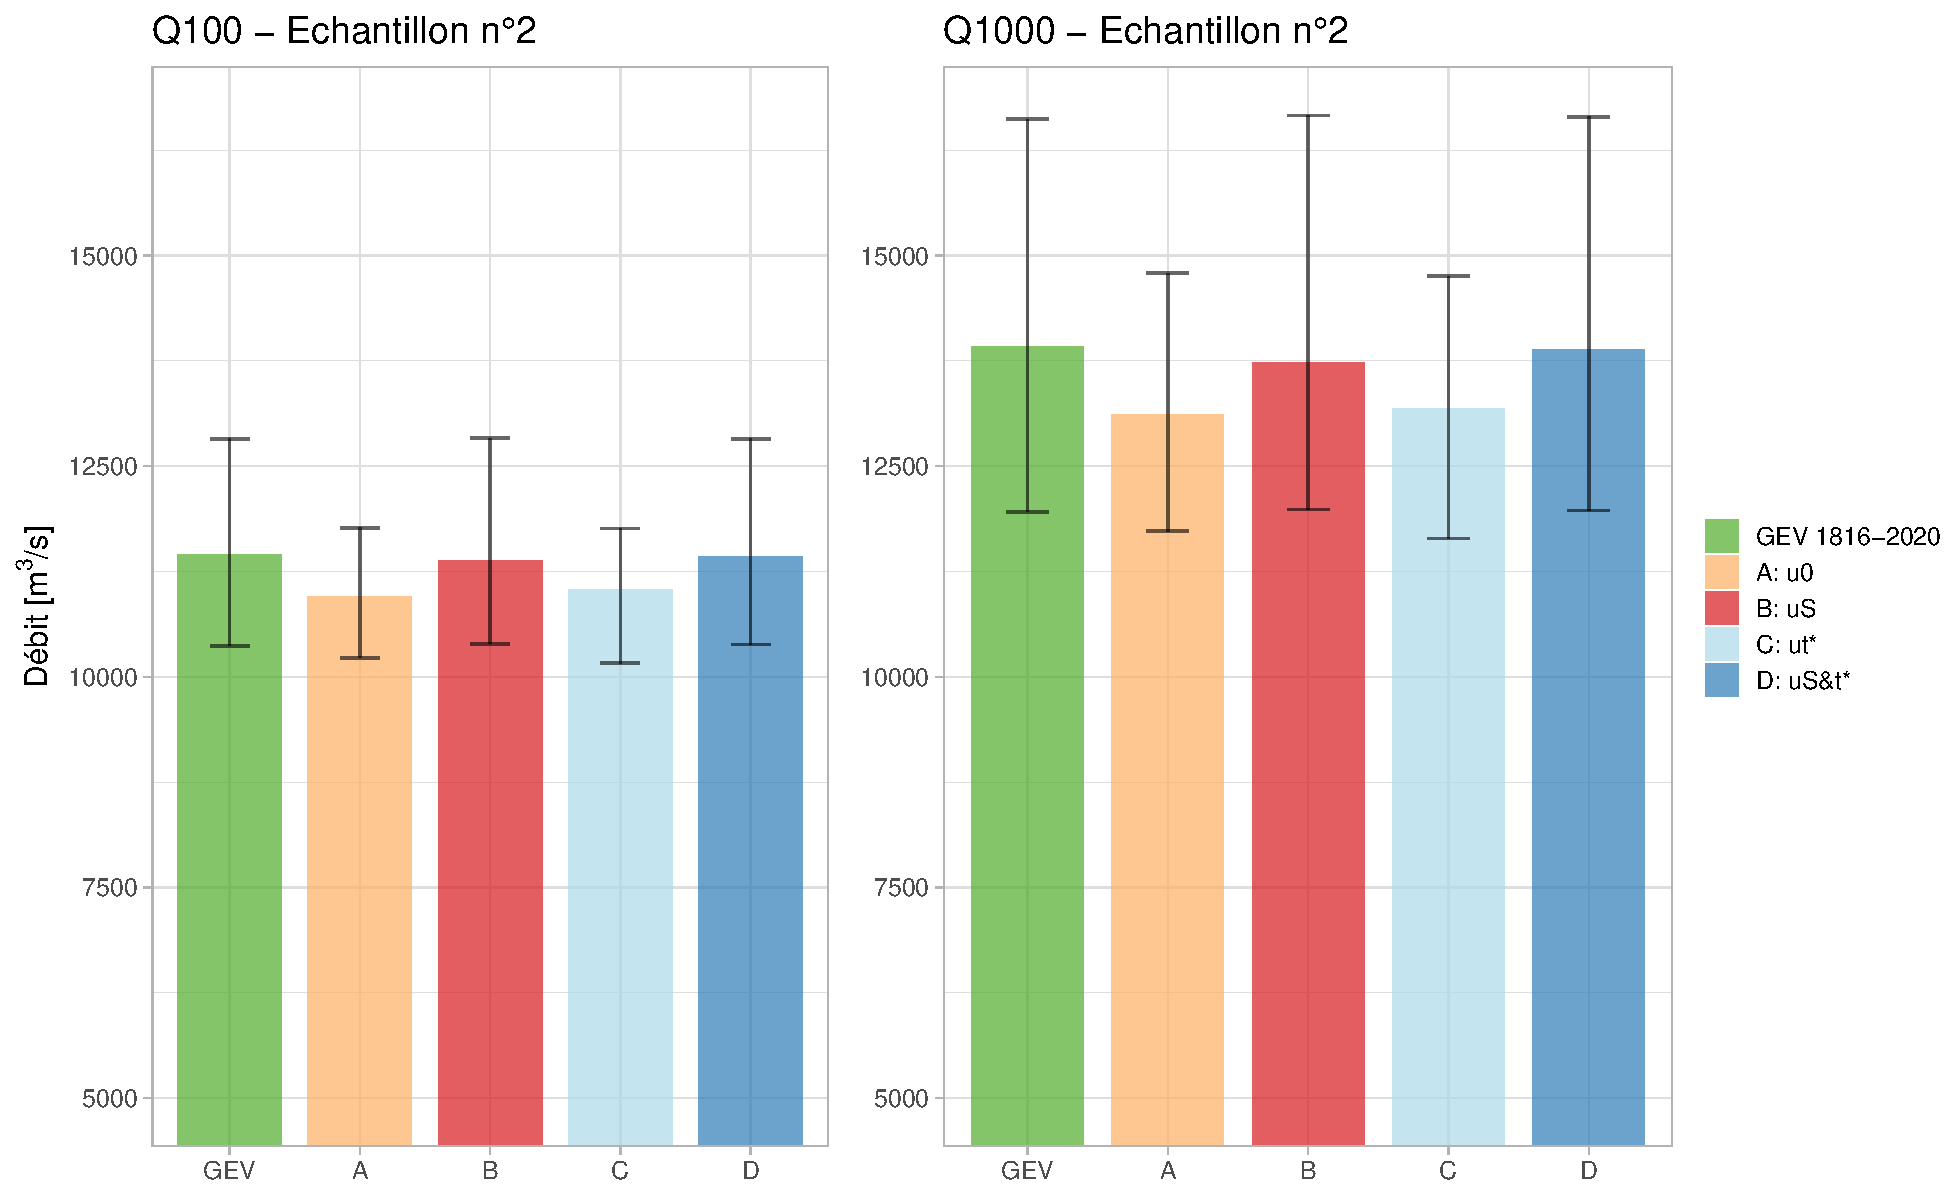
\includegraphics[width=.8\linewidth]{Chapitre4/Figures/Barplots_QX_C4.pdf}
		\caption{Estimations maxpost et incertitudes à 95\% pour Q100 et Q1000 par 5 modèles différents pour l'échantillon 2 (1500-2020, $S4$)}
		\label{fig:BarplotC4}
	\end{figure}
	
		\begin{table}[h]
	\centering
	\caption{Résultats maxpost et incertitudes de 6 modèles pour l'échantillon 2. Le modèle $D^*$ représente les résultats du modèle D avec des a priori plus informatifs (section \ref{subsec:D*}). Q100 et Q1000 représentent respectivement le débit des crues centennales et millénales, $\xi$ le paramètre de forme de la distribution GEV, $S$ le seuil de perception et $t^{*}$ la date de début de la période historique. Les écarts type des distributions a posteriori sont représentés par les colonnes débutant par la lettre "u".}
		\label{tab:ResC4}
	\resizebox{\columnwidth}{!}{%
		\begin{tabular}{|c|c|c|c|c|c|c|c|c|c|c|}
		\hline
Modèle & Q100 [m\textsuperscript{3}/s] & uQ100 [m\textsuperscript{3}/s] & Q1000 [m\textsuperscript{3}/s] & uQ1000 [m\textsuperscript{3}/s] & $\xi$ & $u\xi$ & $S$ [m\textsuperscript{3}/s] & $uS$ [m\textsuperscript{3}/s] & $t^{*}$ & $ut^{*}$ \\ \hline
GEV 1816-2020 & 11451 & 687   & 13919 & 1351   & 0,058 & 0,044  & X    & X    & X    & X \\ \hline
A             & 10977 & 391   & 13149 & 816    & 0,073 & 0,038  & 9000 & X    & 1500 & X \\ \hline
B             & 11438 & 698   & 13875 & 1391   & 0,06  & 0,044  & 9628 & 504  & 1500 & X \\ \hline
C             & 10975 & 395   & 13139 & 809    & 0,074 & 0,038  & 9000 & X    & 1527 & 44 \\ \hline
D             & 11336 & 745   & 13721 & 1467   & 0,061 & 0,044  & 9613 & 551  & 1529 & 62 \\ \hline
$D^*$         & 11118 & 585   & 13421 & 1110   & 0.063 & 0.040  & 9386 & 334  & 1526 & 17 \\ \hline
		\end{tabular}}

	\end{table}
	

	\begin{figure}[h]
		\centering
		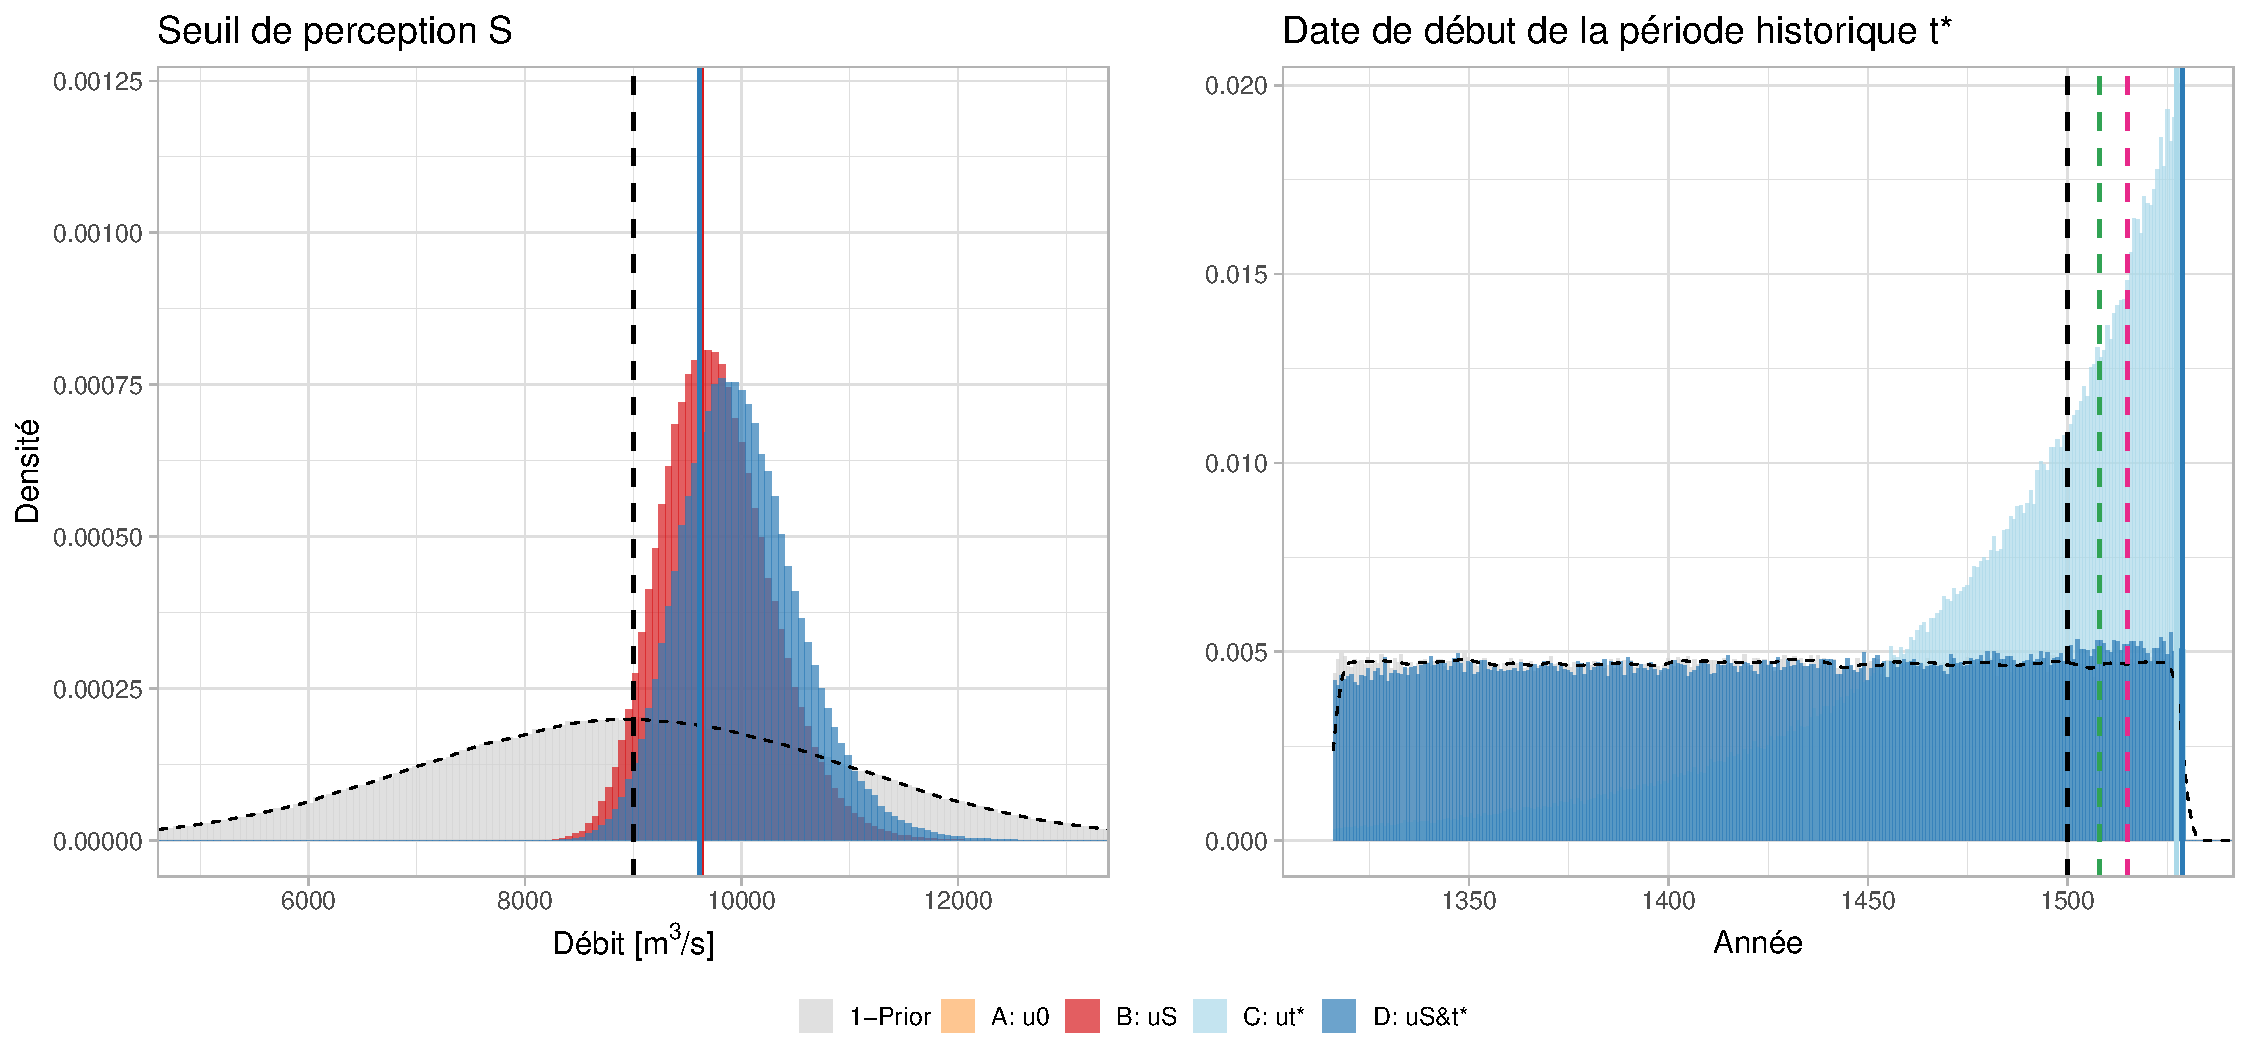
\includegraphics[width=.9\linewidth]{Chapitre4/Figures/Params_C4.pdf}	
		\caption{Distributions a priori et a posteriori pour le seuil de perception (gauche) et la date de début de la période historique (droite). Les droites verticales pleines représentent l'estimation maxpost du paramètre pour chacun des modèles et les droites en pointillés noirs représentent les valeurs de référence. Les droites verticales en pointillés vert et rose représentent respectivement les estimations de $t^{*}$ par la méthode de \citet{prosdocimi_german_2018} et par la méthode de la période de retour du seuil $S$.}
		\label{fig:Params_C4}
	\end{figure}

		\subsubsection{Comparaison des modèles historiques}
		
		
	\paragraph{} Tout d'abord, on observe bien évidemment des résultats moins incertains que pour l'échantillon dégradé (figure \ref{fig:Barplot_Artif2}). L'incertitude des résultats (pour Q100 et Q1000) des modèles GEV-Binomiale est au moins équivalente à celle de la référence (GEV 1816-2020), voire plus faible pour les modèles supposant un seuil de perception connu (A et C). Pour ces mêmes modèles, les quantiles maxpost sont légèrement plus faibles (d'environ 5\%) que ceux de la référence (tableau \ref{tab:ResC4}). De la même manière qu'avec l'échantillon dégradé, on observe ici que la méconnaissance du seuil de perception (B et D) a plus d'impact sur l'incertitude des résultats que la méconnaissance de la durée de la période historique (C et D). 
	
	\paragraph{} On peut notamment expliquer ces différences en observant les distributions a posteriori des paramètres $S$ et $t^{*}$ (figure \ref{fig:Params_C4}). Tout d'abord, ces distributions sont très similaires à celles observées pour l'échantillon 4 (pour des a priori équivalents). Les écarts-type a posteriori pour le seuil de perception (modèles B et D) sont relativement faibles (environ 500 m\textsuperscript{3}/s pour les deux modèles) et les distributions sont centrées vers des valeurs supérieures à la valeur a priori de 9000 m\textsuperscript{3}/s (valeurs maxpost autour de 9600 m\textsuperscript{3}/s, tableau \ref{tab:ResC4}). La date de début de période historique a posteriori pour le modèle C semble à nouveau bien mieux estimée que celle du modèle D, dont la distribution a posteriori est très proche de l'a priori. Pour les deux modèles, les estimations maxpost de $t^*$ sont supérieures de pratiquement 30 ans à la valeur supposée de 1500. On constate notamment que la distribution a posteriori pour le modèle C connait un maximum pour l'année 1529, qui correspond à la date de la première crue de l'échantillon. 
	
	\paragraph{} Cette tendance vers un seuil plus important et une période historique plus courte pourrait être le symptôme d'une non-exhaustivité des crues dans l'échantillon C4 de la base HISTRHÔNE, et ce malgré qu'aucune non-homogénéité de la fréquence des crues supérieures au seuil $S4$ n'ait été détectée (section \ref{subsec:homog}). À nouveau, on peut comparer la fréquence d'occurrence des crues supérieures au seuil $S4$ respective à chacun des deux échantillons. Pour l'échantillon historique, on observe 13 crues pour une durée de 315 ans, soit une fréquence de 0.041 crues/an. Pour l'échantillon continu, on observe 14 crues sur une durée de 204 ans, soit une fréquence de 0.068 crues/an. C'est donc ce déséquilibre en faveur de la période continue, qu'il soit dû à la variabilité d'échantillonnage, à la variabilité climatique, ou à la non-exhaustivité des données historiques, qui entraine l'estimation de seuils de perception plus importants ou de durées historiques plus courtes. L'homogénéité "interne" des deux échantillons a pourtant été validée (section \ref{subsec:homog}), mais cela ne garantit pas une homogénéité inter-échantillons. De plus, il est possible qu'un échantillon soit considéré homogène sans qu'il soit pour autant exhaustif : par exemple la proportion de crues "oubliées" peut être stable dans le temps.
	
	
	\paragraph{} Dans le cas de Beaucaire, l'utilisation du nombre d'occurrences de crues historiques supérieures à un seuil ne permet donc de réduire l'incertitude autour des quantiles estimés que lorsque le seuil de perception est supposé parfaitement connu. L'utilisation d'a priori plus informatifs permettrait probablement d'obtenir des résultats moins incertains et plus réalistes quant à la connaissance du seuil de perception et de la durée de la période historique. Il faut également retenir qu'un doute demeure sur l'exhaustivité de l'échantillon historique ou sur l'homogénéité inter-échantillons.
	 
	 \subsubsection{Estimation des quantiles à Beaucaire (1500-2020) avec des a priori plus informatifs}
	 \label{subsec:D*}

	\paragraph{} Après analyse des résultats des modèles pour différents échantillons, il apparait que l'estimation la plus prudente des quantiles de crues à Beaucaire (1500-2020) consiste à utiliser le modèle D ($S$ et $n$ incertains) en parallèle d'une élicitation d'a priori relativement informatifs. De plus, \citet{stedinger_flood_1986} et \citet{payrastre_usefulness_2011} décrivent qu'un modèle binomial apporte des résultats aussi informatifs qu'un modèle pour lequel le débit des crues historiques est connu si le seuil de perception est suffisamment grand. L'utilisation de l'échantillon correspondant au seuil de perception le plus grand ($S4$) semble donc être plus intéressante. La distribution a priori du seuil est à nouveau supposée gaussienne et centrée sur la valeur de 9000 m\textsuperscript{3}/s, en accord avec les estimations de \citet{pichard_hydro-climatology_2017} et des résultats du chapitre \ref{chap:ch2}. L'écart type de la distribution est fixé à 500 m\textsuperscript{3}/s, ce qui le rend l'a priori plus informatif que lors des calculs précédents. En ce qui concerne la date de début de la période historique $t^{*}$, une distribution uniforme est utilisée. La borne supérieure de la distribution reste fixée à la date de la première crue de la série (en 1529). En revanche, la borne inférieure est affectée à deux fois la durée entre la date de la première crue (1529) et la valeur supposée de $t^{*}$ (1500), soit 58 ans. La borne inférieure de la distribution a priori est donc l'année 1471. La valeur théorique calculée en utilisant la méthode proposée par \citet{prosdocimi_german_2018} est 1510, elle est bien comprise dans la distribution a priori. Il en est de même pour la valeur de $t^{*}$ correspondant à la différence entre la période de retour du seuil de perception $S4$ (environ 15 ans) et la date de la première crue, ce qui correspond à l'année 1515. L'application du modèle D avec ces a priori plus informatifs correspondra au terme $D^*$ dans les sections suivantes

	\begin{figure}[h]
		\centering
		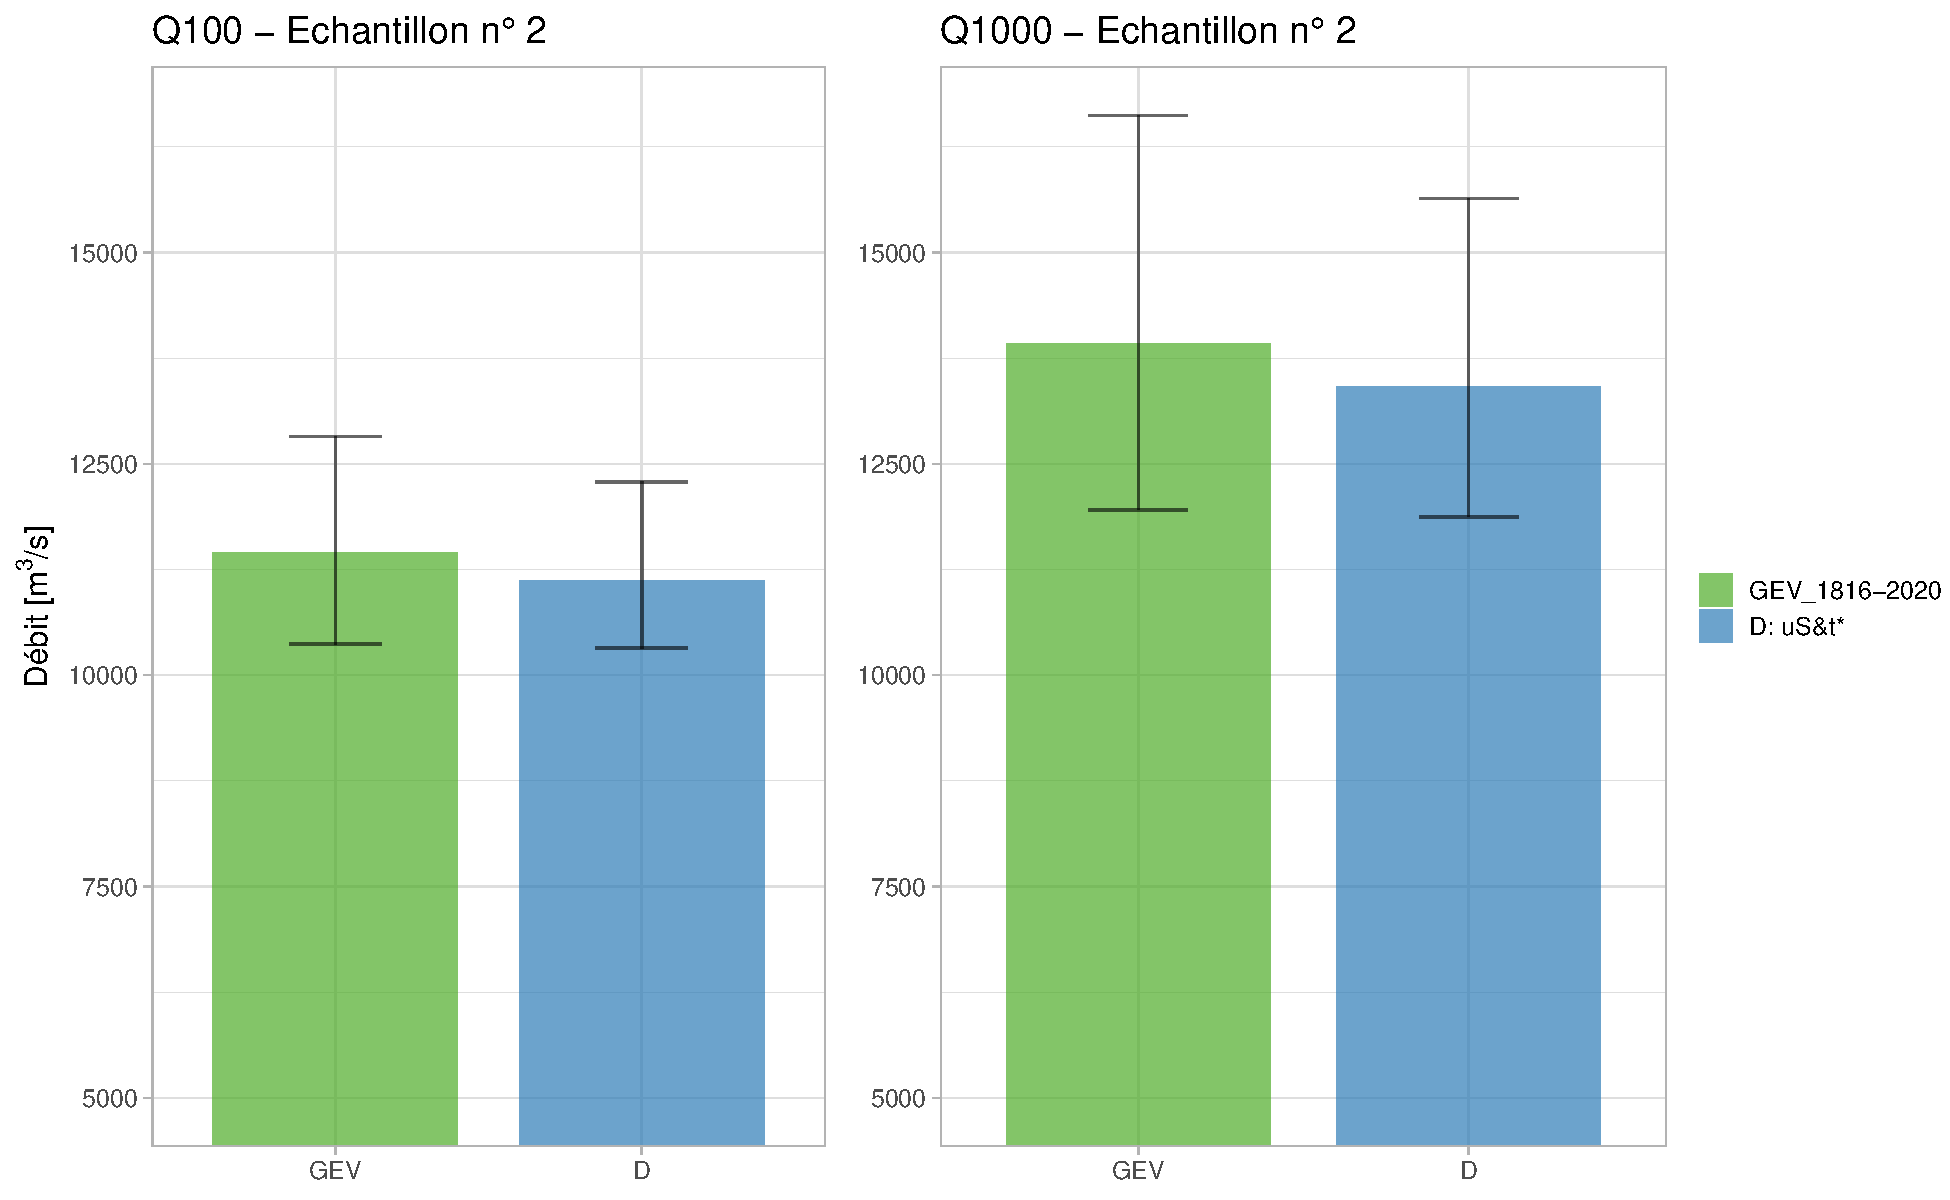
\includegraphics[width=.8\linewidth]{Chapitre4/Figures/Barplots_QX_C4short.pdf}
		\caption{Estimations maxpost et incertitudes à 95\% pour Q100 et Q1000 des modèles GEV 1816-2020 et $D^*$ pour l'échantillon 2 (1500-2020, $S4$) après révision des distributions a priori de $S4$ et $n$.}
		\label{fig:BarplotC4short}
	\end{figure}

	\paragraph{} Les résultats du modèle $D^*$ sont présentés dans la figure \ref{fig:BarplotC4short} ainsi que dans le tableau \ref{tab:ResC4} où ils sont comparés avec les estimations de référence (GEV 1816-2020). On constate que l'incertitude des quantiles est réduite d'environ 15\% par rapport à la référence pour Q100 et Q1000. Les estimations maxpost sont également réduites d'environ 3\% pour les deux périodes de retour. L'utilisation des crues historiques apparait donc pertinente pour réduire l'incertitude des quantiles, même dans le cas où $S$ et $n$ sont incertains. On peut également noter que l'élicitation d'a priori plus informatifs a permis de réduire d'environ 25\% l'écart type de la distribution a posteriori pour Q1000 (comparaison de D et $D^*$). 

%	\begin{table}[h]
%	\centering
%	\caption{Résultats maxpost et incertitudes de 2 modèles pour l'échantillon 2 après révision des distributions a priori de $S4$ et $n$. Q100 et Q1000 représentent respectivement le débit des crues centennales et millénales, $\xi$ le paramètre de forme de la distribution GEV, $S$ le seuil de perception et $t^{*}$ la date de début de la période historique. Les écarts type des distributions a posteriori sont représentés par les colonnes débutant par la lettre "u".}
%	\label{tab:ResC4short}
%	\resizebox{\columnwidth}{!}{%
%		\begin{tabular}{|c|c|c|c|c|c|c|c|c|c|c|}
%		\hline
%Modèle & Q100 [m\textsuperscript{3}/s] & uQ100 [m\textsuperscript{3}/s] & Q1000 [m\textsuperscript{3}/s] & uQ1000 [m\textsuperscript{3}/s] & $\xi$ & $u\xi$ & $S$ [m\textsuperscript{3}/s] & $uS$ [m\textsuperscript{3}/s] & $t^{*}$ & $ut^{*}$ \\ \hline
%GEV 1816-2020 & 11451 & 687   & 13919 & 1351   & 0.058 & 0.044  & X    & X    & X    & X \\ \hline
%
%		\end{tabular}}
%
%	\end{table}
		
	\paragraph{} Les distributions a posteriori de $S$ et $t^{*}$ sont présentées dans la figure \ref{fig:Params_C4short}. Une fois de plus, la distribution a posteriori du seuil de perception est décalée vers des valeurs plus élevées que la valeur supposée de 9000 m\textsuperscript{3}/s, avec un seuil maxpost à 9386 m\textsuperscript{3}/s. La distribution a posteriori de $t^{*}$ est à nouveau très proche de la distribution a priori, avec une densité un peu plus élevée pour les années proches de la date de la première crue. L'estimation maxpost de $t^{*}$ est ici 1526, soit une durée de la période historique $n$ 26 ans plus courte qu'attendu. Cependant, le doute quant à l'exhaustivité de l'échantillon historique ou l'homogénéité inter-échantillons tel que décrit dans la section précédente.
			
	\begin{figure}[h]
		\centering
		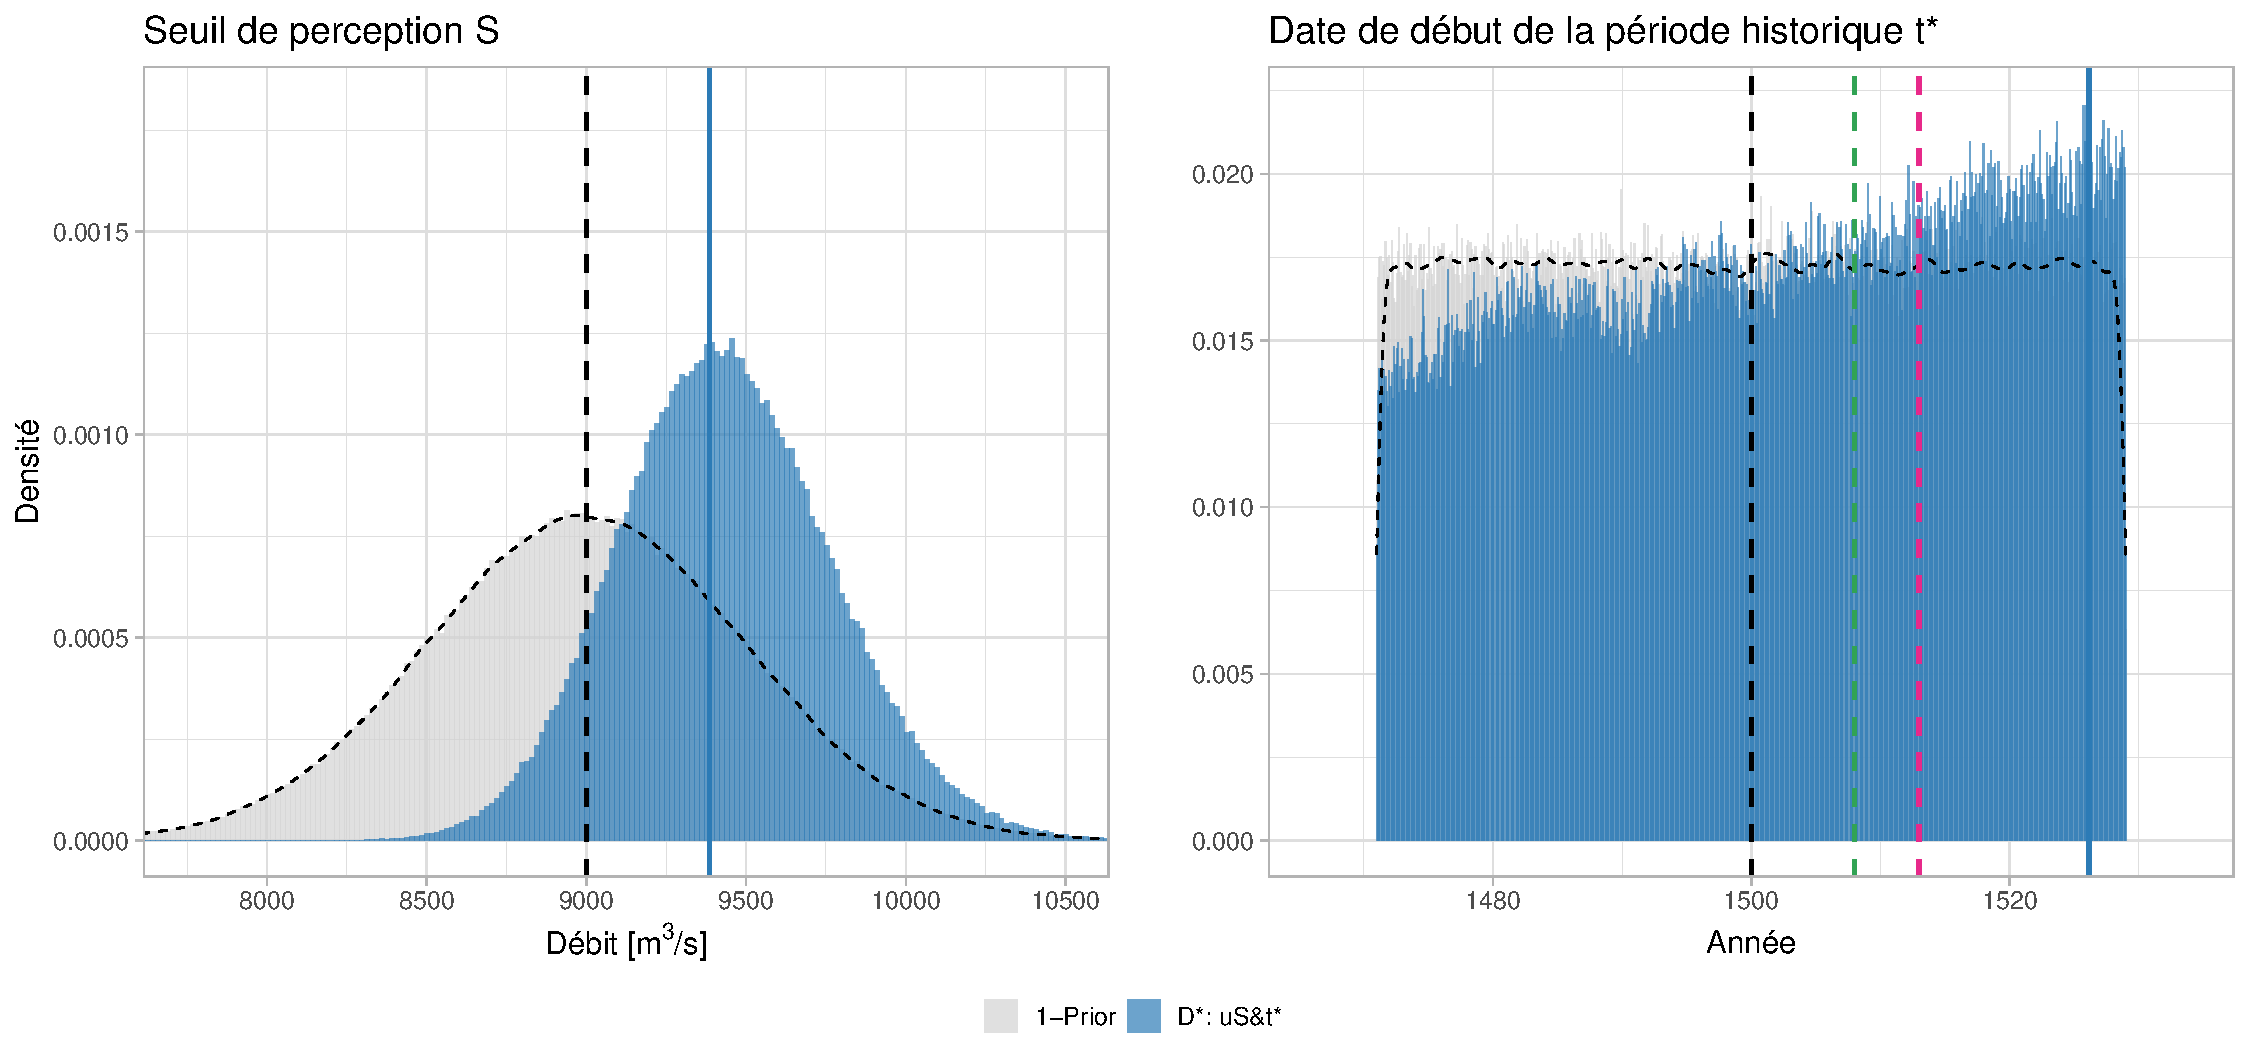
\includegraphics[width=.9\linewidth]{Chapitre4/Figures/Params_C4short.pdf}	
		\caption{Distributions a priori et a posteriori pour le seuil de perception (gauche) et la date de début de la période historique (droite). Les droites verticales représentent l'estimation maxpost du paramètre de forme pour chacun des modèles. La droite verticale noire représente la date de début supposée de la chronique historique, ici 1500.}
		\label{fig:Params_C4short}
	\end{figure}
	
	\FloatBarrier
	
	\section{Discussion}
	\label{sec:Discussion}
	\paragraph{} L'intérêt de la valorisation des données historiques pour l'analyse fréquentielle des crues est connu et étudié depuis longtemps (\cite{benson_use_1950}; \cite{stedinger_flood_1986}). L'utilisation des données anciennes doit être accompagnée d'une estimation complète des incertitudes \citep{kjeldsen_documentary_2014}. Lors de l'utilisation d'un échantillon d'occurrences de crues supérieures à un seuil (le débit des crues historiques supérieures au seuil de perception n'est pas connu), la méconnaissance du seuil de perception et de la durée de la période historique est souvent négligée. Seule l'incertitude provenant de l'estimation des paramètres de la distribution choisie est généralement considérée. Plusieurs modèles sont proposés dans ce chapitre permettant de prendre en compte la méconnaissance autour de ces deux paramètres. La propagation de l'incertitude des débits de la période récente est également effectuée. 
	
	\paragraph{} Les modèles ont dans un premier temps été testés avec des a priori très peu informatifs et sur un échantillon continu artificiellement dégradé afin de se replacer dans un contexte historique. Ainsi, seuil de perception et durée de la période historique sont parfaitement connus. Les quantiles estimés ont été comparés avec les estimations d'un modèle GEV pour l'entièreté de la période (figure \ref{fig:Barplot_Artif2}). Il est apparu que considérer le seuil de perception comme étant incertain avait bien plus d'impact sur l'incertitude des résultats que considérer une méconnaissance sur la durée de la période historique. En revanche, quand ces deux paramètres sont considérés incertains en même temps, l'incertitude autour des quantiles est réduite par rapport au cas où seul le seuil est incertain. Une corrélation entre les distributions a posteriori de ces deux paramètres a été mise en évidence. Cette corrélation n'est pas surprenante étant donné que seuil et durée de la période historique sont par définition reliés : le nombre de dépassements du seuil de perception $k$ est à la fois dépendant du seuil $S$ et de la durée $n$. L'élicitation d'a priori plus informatifs pour ces deux paramètres est donc nécessaire. Bien que le seuil de perception soit un objet parfois difficile à cerner, il est donc possible de représenter sa méconnaissance à l'intérieur même du modèle probabiliste. Considérer que le seuil de perception est parfaitement connu lorsque ce n'est pas le cas peut mener à une importante sous-estimation de l'incertitude des quantiles, de même que pour la durée de la période historique, dans une moindre mesure. Dans le cas de cet échantillon dégradé, l'utilisation des données historiques permet de réduire l'incertitude des quantiles par rapport à la seule utilisation de l'échantillon continu (dégradé), et ce quelque soit l'hypothèse retenue concernant la méconnaissance de $S$ et $n$.
	
	\paragraph{} L'estimation du modèle binomial pour $S$ et $n$ connus (modèle A) a ensuite été comparée à une estimation pour laquelle le débit des crues historiques est connu et situé dans un intervalle (modèle E) pour l'échantillon dégradé (figure \ref{fig:CensureArtif}). L'incertitude des résultats du modèle E se situe entre celle du modèle A et celle du modèle GEV pour l'ensemble de la période. Dans ce cas précis, l'utilisation du débit des crues historiques s'est donc avérée légèrement plus informative que l'utilisation du seul nombre de dépassements du seuil de perception. D'après \citet{stedinger_flood_1986} et \citet{payrastre_usefulness_2011}, la magnitude du seuil de perception utilisé influe directement sur l'incertitude des résultats dans le cas du modèle binomial. Ainsi, pour un seuil de perception suffisamment grand, l'incertitude des estimations du modèle binomial est identique à celle du modèle pour lequel le débit des crues historique est connu. L'intérêt de connaitre précisément le débit des crues historique est moindre dans ce cas. \citet{payrastre_usefulness_2011} estiment que l'on se trouve dans cette situation lorsque la période de retour du seuil de perception est supérieur à environ 50 ans (dans les cas testés). A Beaucaire, la période de retour du seuil de perception $S4$ est d'environ 15 ans, ce qui explique l'avantage du modèle E sur le modèle A dans ce cas précis.
	
		\paragraph{} Pour l'échantillon de crues de Beaucaire de 1500 à 2020, l'utilisation des données anciennes reste, en l'absence d'estimations du débit des crues historiques, conditionnée à l'utilisation des seuils de perception de la base HISTRHÔNE : $S3$ ou $S4$. L'estimation des quantiles étant plus précise pour un seuil de perception correspondant à une période de retour importante, il est naturel de préférer le seuil $S4$. Il parait également plus prudent d'utiliser le modèle qui fait l'hypothèse d'une méconnaissance du seuil de perception et de la durée de la période historique (modèle D), en parallèle d'une élicitation réaliste des a priori de ces deux paramètres. Les résultats du modèle D sous les conditions décrites précédemment sont légèrement plus informatifs que l'utilisation de la seule chronique continue de 1816 à 2020 (figure \ref{fig:BarplotC4short}). Néanmoins, des doutes subsistent sur l'exhaustivité de l'échantillon historique. 
	
	\paragraph{} L'application des quatre modèles à l'échantillon complet de 1500 à 2020 à Beaucaire avec des a priori peu informatifs a montré que les estimations de la durée historique et du seuil de perception étaient différentes des valeurs supposées. Les modèles B et D estiment un seuil de perception plus grand que supposé et les modèles C et D estiment une durée de la période historique légèrement plus courte que celle supposée (figure \ref{fig:Params_C4}). Cette tendance pourrait être le symptôme d'une non-exhaustivité des crues dans les échantillons historiques de la base HISTRHÔNE, et ce bien qu'aucune non-homogénéité de la fréquence des crues n'ait été détectée (section \ref{subsec:homog}). Le nombre $k$ de dépassements du seuil de perception est donc possiblement sous-estimé dans les données disponibles. Cette sous-estimation pourrait provenir de la nature même des données, qui ne sont pas des données de crues supérieures à un seuil au sens physique. Les catégories de la base HISTRHÔNE sont définies sur la perception des dommages par les populations ripariennes et non un seuil de perception physique directement lié au dépassement d'un débit. Or, comme décrit au chapitre \ref{chap:ch2}, la perception des dommages par les populations a probablement évolué au cours du temps. Cette variabilité dans la perception des dommages et la conséquence de nombreux facteurs, qu'ils soient physiques ou anthropiques. Ainsi, relier directement les conséquences d'une crue à son seul débit de pointe est un raccourci dangereux. Par exemple, pour un même débit de pointe, la perception de la gravité d'une crue peut varier selon la durée de la crue, le niveau de protection, la rupture de digues, la densité de population... De plus, la qualité et la quantité des témoignages de crues historiques qui parviennent jusqu'à nous sont dépendants du contexte sociétal, qui est lui aussi très variable d'une époque à l'autre : contexte politique, religieux, médiatique, culture de la conservation d'archives... Par exemple, l'impressionnante quantité de données recueillie dans la base HISTRHÔNE est notamment la conséquence de la présence d'instances religieuses dans la région provençale, au sein desquelles l'érudition et la tradition écrite étaient importantes. Cet ensemble de paramètres est important à garder en tête lors de l'utilisation de données historique pour l'analyse fréquentielle, et plus particulièrement lors de la phase d'enquête historique. La méthodologie de la recherche de données est tout aussi importante que l'analyse statistique, afin de garantir l'exhaustivité des échantillons et la connaissance du contextes hydrologique, hydraulique et social contemporain aux crues étudiées. 	
	
	\paragraph{} Dans les études historiques menées sur des bassins versants français de petite taille, la détermination du seuil de perception $S$ et l'exhaustivité du nombre de crues $k$ supérieures au seuil semblent être les principales limites. Par exemple, \citet{payrastre_possibility_2005} écrit : «\textit{De façon à disposer d'une information fiable nous avons parfois dû limiter la durée de la reconstitution historique à moins de deux siècles (durée visée au départ), un seuil de perception ne pouvant raisonnablement être défini}». Il en est de même pour les données de la base HISTRHÔNE utilisées ici et dont les plus anciens témoignages remontent au XIII\textsuperscript{ème} siècle. L'avis d'expert de Geoges PICHARD, l'historien à l'origine de cette base de données, était que l'exhaustivité des crues était probablement atteinte à partir du XVI\textsuperscript{ème} siècle, ce qui nous a conduits à utiliser les données de la base à partir de l'année 1500. Ce constat était sans doute optimiste et nous avons été confortés dans ce choix par les résultats l'analyse de stationnarité réalisée à la section \ref{subsec:homog}. On pourrait penser que choisir début de période historique plus tardif aurait pu mener à de meilleurs résultats. Cependant, le fait que l'homogénéité de l'échantillon historique ait été validée semble suggérer que la fréquence des "oublis" de crues supérieures au seuil soit constante au cours du temps. Il est risqué de vouloir à tout prix utiliser le plus grand nombre de données historiques possible dans un contexte d'analyse fréquentielle. L'exhaustivité doit être le premier critère, devant la quantité de données utilisée. Par exemple, \citet{gaume_bayesian_2010} écrivent dans un contexte légèrement différent d'analyse historique et régionale des crues : «\textit{comprehensive and dense inventories of ungauged extremes with a controlled and predefined number of target watersheds not selected on the basis of the magnitude of the past floods (French example), should be preferred to loose collations of isolated extreme values with unknown equivalent coverage. For a given series, if there is an uncertainty on the threshold values, the highest guesses should be selected to obtain the pessimistic result concerning the credibility bounds.}»
	
	\paragraph{} Suite à ces différents constats, on pourrait penser à l'utilisation d'un modèle qui considère non-seulement le seuil de perception $S$ et la durée de la période historique $n$ comme étant incertains, mais également pour lequel le nombre de dépassements $k$ du seuil de perception est lui aussi incertain. Néanmoins, les résultats de ce chapitre ont permis de mettre en évidence que la méconnaissance de $S$ avait à elle seule un fort impact sur les résultats. De plus, lorsqu'il existe un tel doute sur l'exhaustivité des données historiques, discuter de l'incertitude du seuil de perception ou de la durée de la période historique parait secondaire. Ici, l'utilisation même des données historiques pourrait être remise en cause, l'échantillon d'enregistrements continus étant exceptionnellement long (205 ans) et permettant une estimation satisfaisante des quantiles de crue. Une des façons de compléter cette étude pourrait être d'estimer le débit des événements historiques à l'aide de modèles hydrauliques avec une prise en compte complète des incertitudes inhérentes à cet exercice (bathymétrie historique, rupture de digues...) listées dans le chapitre \ref{chap:ch2}. Cependant, cela ne réglerait pas les problèmes de non-homogénéité énoncées plus tôt. Il est également possible d'utiliser plusieurs seuils de perception dans le but de garantir l'exhaustivité des données pour les périodes les plus anciennes. Cette possibilité est fréquemment décrite dans la littérature mais n'a jamais été exploitée dans le cas de seuils de perception incertains. Considérer plusieurs seuils de perception incertains en parallèle avec des durées de périodes incertaines peut néanmoins nécessiter un traitement statistique bien plus complexe que celui décrit dans ce chapitre.
	
	\paragraph{} Bien que l'homogénéité des données ait été vérifiée (section \ref{sec:dataBcr}), il est probable que les données utilisées dans ce chapitre soient impactées par une variabilité climatique et/ou anthropique qui pourrait fragiliser l'hypothèse de stationnarité nécessaire à l'analyse fréquentielle. L'hypothèse de stationnarité est de nos jours fréquemment remise en cause \citep{milly_stationarity_2008}. Des tendances autour de la magnitude des crues ont été identifiées dans plusieurs régions en Europe (\cite{hall_understanding_2014}; \cite{bloschl_changing_2019}) et en France \citet{giuntoli_floods_2019}, mais aucune règle n'existe en France à ce jour pour prendre en compte l'impact du changement climatique sur l'estimation du risque inondation \citet{madsen_review_2014}. Néanmoins, la non-prise en compte de ces sources de variabilité a probablement moins d'impact sur les résultats que la méconnaissance autour des données historiques et la simple variabilité d'échantillonnage. Il est tout de même possible d'intégrer les changements temporels des processus climatiques ou des caractéristiques du bassin versant au sein même du modèle probabiliste comme cela est de plus en plus fréquemment décrit dans la littérature (voir \citet{salas_techniques_2018} pour une revue complète des différentes possibilités). Il ne faut pas oublier que cette longue série est utile en dehors du cadre de l'analyse fréquentielle. Il est possible de l'utiliser pour identifier la variabilité climatique sur les 5 derniers siècles. On peut citer à ce sujet les résultats de \citet{bloschl_current_2020}, basés sur de plus de 100 séries historiques de crues provenant de diverses régions européennes. Ces derniers ont mis en évidence plusieurs périodes au cours des 500 dernières années durant lesquelles la fréquence d'occurrence des crues était amplifiée. Ils ont également montré que la période actuelle (1992-2016) était l'une de ces périodes riches en crues et qu'elle était inédite par rapport aux autres périodes, notamment en terme d'extension spatiale du phénomène. 
	
	
	\paragraph{} Les conclusions de ce chapitre ne sont difficilement généralisables à d'autres stations que Beaucaire, notamment pour des régions climatiques sous des influences différentes ou des bassins versants plus petits. La réduction de l'incertitude, en partie dépendante du comportement de la queue de distribution (et donc du paramètre de forme de la GEV), serait probablement différente sous un autre contexte climatique, tout particulièrement dans le cas d'une queue de distribution plus "lourde" que celle de Beaucaire \citep{merz_understanding_2022}. Il est également probable que la réduction d'incertitude obtenue par l'utilisation de données historiques soit dépendante du ratio des durées de la période historique et de la période continue \citep{payrastre_usefulness_2011}. De plus, on peut également s'attendre à des résultats différents selon la nature des données historiques utilisées (témoignages, repères de crues, dendrochronologie, carottes sédimentaires...). L'application des méthodes proposées dans ce chapitre à d'autres stations hydrométriques, comportant des données historiques exhaustives et de nature différente à celles de Beaucaire serait intéressante. Pour que les résultats soient comparables, l'estimation et la propagation de l'ensemble des incertitudes devra être effectuée. 
		
	
\section{Conclusion du chapitre}
\label{sec:Conclu}
	\paragraph{} La méconnaissance du seuil de perception et de la durée de la période historique est quasi-systématiquement négligée lors de l'utilisation de données historiques. Les modèles mis au point dans ce chapitre permettent de considérer cette méconnaissance au sein même du modèle probabiliste et de la propager aux résultats. Il est apparu en testant les modèles sur une chronique artificiellement dégradée que la méconnaissance du seuil de perception avait plus d'impact sur l'incertitude des résultats que la méconnaissance de la durée de la période historique. De plus, une corrélation entre ces deux paramètres a été mise en évidence. L'utilisation de la chronique complète (1500-2020) a ensuite permis de réduire l'incertitude les estimations des quantiles extrêmes réalisées au chapitre \ref{chap:ch3}, même dans le cas où seuil de perception et durée de la période historiques sont incertains, à condition d'utiliser des a priori suffisamment informatifs. Cependant, cette application a également permis de mettre en lumière une probable sous-estimation du nombre de dépassements du seuil de perception au cours de la période historique. Considérer une incertitude autour de $S$ ou $n$ est probablement mineur devant le problème de la non-exhaustivité des données historiques.

	\paragraph{} On peut donc retenir que, malgré la non-exhaustivité supposée de l'échantillon, ces résultats soulignent l'intérêt potentiel de l'utilisation des données historiques pour l'analyse fréquentielle, ainsi que l'importance d'une prise en compte complète des incertitudes autour de ces données. Ces conclusions ne sont pas systématiquement généralisables en dehors du cas de Beaucaire, où la chronique d'enregistrements continus est particulièrement longue et où le paramètre de forme est positif. De plus, aucune tendance pouvant être attribuée aux changements des caractéristiques du bassin versant ou au changement climatique n'a pu être mise en évidence à Beaucaire. Néanmoins, pour aller au delà de l'analyse fréquentielle des crues, la perspective de modéliser la variabilité climatique semble intéressante avec un jeu de données aussi fourni.

%\newpage
%
%\printbibliography[title=Bibliographie]
%\end{document}
